\documentclass[11pt,a4paper]{jreport}
%
\usepackage{amsmath,amssymb}
\usepackage{bm}
\usepackage{graphicx}
\usepackage{ascmac}
\usepackage{float}
%
\setlength{\textheight}{40\baselineskip}
\addtolength{\textheight}{\topskip}
\setlength{\voffset}{-0.2in}
\setlength{\topmargin}{0pt}
\setlength{\headheight}{0pt}
\setlength{\headsep}{0pt}

\setlength{\textwidth}{\paperwidth}     % ひとまず紙面を本文領域に
\setlength{\oddsidemargin}{-5.4truemm}  % 左の余白を20mm(=1inch-5.4mm)に
\setlength{\evensidemargin}{-5.4truemm} % 
\addtolength{\textwidth}{-40truemm}     % 右の余白も20mmに
%
\newcommand{\divergence}{\mathrm{div}\,}  %ダイバージェンス
\newcommand{\grad}{\mathrm{grad}\,}  %グラディエント
\newcommand{\rot}{\mathrm{rot}\,}  %ローテーション
%
\title{脳を学ぶ上で重要な数学シリーズ}
\author{後藤 優仁}
\date{\today}
\begin{document}
\maketitle
%
%
\tableofcontents


\section{本書の目的}
慶應義塾において, 塾生同士の繋がりは尊ぶべきであり, その立場に関わらず学び教えあう 半学半教 の精神が大事であると福澤先生は仰っております. \\
\\
よって僕も, 未熟者ではありますが後進の育成のため, ひいては将来僕に教えてくれうる人材への先行投資として, はたまた自分の復習用にこの資料を作成することにしました. 脳は学ぶ事はあまりにも難しく, 脳を学ぶ事で脳を病んでしまうものですが, ともに頑張りましょう! \\
\\
最初にことわっておくと, 本書ではある程度までの分かりやすさを担保しますが, 逆にある程度以上は「自明」で片づけます. 初学者はもちろん「自明じゃねえよふざけんな!」と思う事でしょうが, このイラ立ちが大事なのです. 自明なものを自明と思えないという事は, 読者の理解力・基礎力が足りていないという事です. \\\\
分からなかった単語や数式をググり, 本を借り, 先生や先輩に聞き, 手計算で確認し, 実装してプロットした結果を眺める...このようにして崇める事で, いつしか調べていた事が自明であった事に気付けるようになります. 中学数学に対して「自明じゃねえよ」なんて考える人はいませんね?それと一緒です.\\
\\
\\
さて筆者のプロフィールですが, 脳神経科学歴1年, 数学歴半年のペーペーです. 数学に至っては半年前は虚数が何か分からなかったし三角関数の意味も知りませんでした.\\
よって変な理解だとか知識の抜けもあると思うのでご指摘お待ちしています.\\
\\
最初の節は, 僕が初めて数学にしっかりと向き合うきっかけになった, 僕の先生がくださった資料を改変したものです. しかし, 僕はこの元となる資料をもらった当初は何一つ解読不能でした. よって, その内容を理解するために独学で補った知識がそれ以降の節にまとめてあります. 自信がない単元があったら復習をしてみてもいいかもしれません. \\
\\
\section{本書のカバーする内容}
本書は筆者の気が向いた時に少しずつ更新していくので, タイミングによってはほとんど書いてないと思いますが, 最終的に目指している点をここに記します.\\
\\
基本的には脳神経科学, 特に脳波を用いる際に必要になってくる数学を全体集合として, 部分集合を小出しにだしていく感じを考えています. 補集合については更新を待つか諦めて独学をする, あるいは筆者に書くよう申請をしてください. 従って本書のカバーする内容はおおまかに分けて\\
\\
\begin{itemize}
 \item 前提となる基礎的な数学
 \item 脳波を代表とした信号を処理する信号処理数学
 \item ANOVAやt検定, 簡単な機械学習などの統計的数学
\end{itemize}

などといった感じになると思います. 軟弱なSFC生の多くはいらないと考えるでしょうが, 少なくとも他大学の脳科学の研究室ではどれも児戯のごとき基礎となっています(実際学部1.2年で大体習ってる). がんばりましょう.
\\
\\
\chapter{基礎を学ぶ \label{basics}}
\section{掛け算}
\subsection{掛け算とは何か}
掛け算とはとても難しいものです.\\
何故なら, 足し算はユークリッド空間から離れた複雑な空間でも, 大抵は普通にこなすことが出来ますが, 掛け算はユークリッド空間をほんの少し離れてしまっただけで難解になってしまうからです. \\
\\
逆に言うと足し算では違いが分からない様々な空間も, 掛け算で考えると全く異なる空間であった事が理解できるとも言えます. ベクトルや行列の事です.\\
ちなみに, 割り算になると難しすぎて頭が爆発します. 逆行列の考え方の事です. \\
引き算が足し算で表せるのは自明なので割愛(割り算も掛け算で表せるだろと思った君, そうもいかない奴らもいるのだ.)\\
信号処理や統計の勉強をしていくには, 掛け算は非常に大切なものです. まずは掛け算の偉大さと深淵に触れましょう.\\
\\
\subsubsection{数ってなぁに?}
先程, ユークリッド空間やらなんやらといった言葉が出てきましたが, 簡単にいうとこれらは全て別の「数」として考える必要があるため, 空間と名付けています.\\
まずは単一の数と複数の数に分けるところからいきましょう.\\

\subsubsection{単一の数スカラー}
単一の数, スカラー数です. 高校での数学を真面目に受けていた人間なら聞き覚えがえるでしょう. スカラー数とは最も簡単な数...すなわち僕達が昔から親しんできた「数」のことです!\\
簡単ですね!以上です.\\
\\
スカラー数の掛け算は僕たちが直感的にやっている
\begin{eqnarray}
3 * 5 = 15
\end{eqnarray}

の事です.
\\

\subsubsection{複数の数からなる積}
複数の数からなる数には色々あります.\\
\begin{itemize}
 \item ベクトル
 \item 複素数
 \item 行列
\end{itemize}

等です. これらはスカラー数の掛け算とは全く違う世界になります. 心してかかりましょう. 高校以上の数学は非常に難しいもので, 僕も全く分からずに置いて行かれましたが, どうにか理解するための最初の第一歩は, 「世の中には(スカラー)数じゃない数があるらしい」と知る事です. 僕はこれを理解するまでに4年の歳月を費やしてしまいました. \\
\\
では, そもそも何故スカラー以外の数を考える必要があるのでしょうか?\\
普通に生きていてベクトルや複素数といったものを自然の中に見る事はないでしょう(あるいは啓蒙を高めると見る事が出来るのやもしれない).\\
しかしスカラー数には限界があるのです. 何故なら, 基本的にスカラー数とは直線であるからです! \\
\\
0があって1があり, その次に2が来るのは小学2年生の数直線ですが, 小学4年生頃には「どうやら0と1の間にも小数や分数があるらしい」と知ります. 次に中学になり, 0の向こう側には同じだけの数の負の数があり, 更には√がつく数などもある事を知ります. そして少し飛びますが高校では, 数直線の右と左に終わりはなく, 無量大数という領域に飛んでいる事を知りますね. ここまでがスカラーの学習順序ですが, いずれも1本の直線を細かく見たり, あるいはずっと先を見ているだけです. \\
\\
ただの直線であるスカラーでは記述できる情報が少ないため, 不都合があるから別の数を考える必要があったわけです. スカラーっぽいやつらを複数束ねてまとめた「数」を新しく定義してやれば表現できる情報量は各段に増え, 世界が広がります. \\
\\
記述する要素が増えれば情報が増えるのは自明ですね. 
\\
\subsubsection{ベクトルの積}
ベクトルとは, 二次元の場合は2つ, 三次元の場合は3つの数を束ねたものです. \\
数を複数束ねると, その間に比が生まれ, 角度 (とそれによる長さ) が生まれます. \\
これが先述した, 増える情報量であり, スカラー数との決定的な違いです.\\
ちなみに, この「比と角度と長さ」ですが, これは脳波においては位相やフィルター, 電位の強度といったものを考える時に必要になります. というかそのままです. 図に書いてよく確認しておいてください. 
\\
ベクトル同士を掛け合わせるとき, どうするでしょうか?\\
一番素朴な形は下記の通りでしょう.\\
\begin{eqnarray}
(\mathstrut x_1 , \mathstrut y_1)(\mathstrut x_2 , \mathstrut y_2 ) = (\mathstrut x_1 \mathstrut x_2 + \mathstrut y_1 \mathstrut y_2)
\end{eqnarray}

これをベクトルの内積と言います.\\
そして, ベクトルの内積はもう一つの算出方法がありましたね. 2つのベクトルの絶対値の積に互いになす角の cos をかけたものです. 確認してみましょう.\\
\\
ある2つのベクトルを考えてください.\\
1つは $(\mathstrut r_1\cos x , \mathstrut r_1\sin x)$ で, もう一つは 
$(\mathstrut r_2\cos y , \mathstrut r_2\sin y)$ です.
\\
全ての比は cosx:sinx で表せるので上記の表し方は問題ありません (参照: \ref{trigonometry}).\\
\\
では内積を考えます.\\
\\
\begin{eqnarray}
(\mathstrut r_1\cos x, \mathstrut r_1\sin x)(\mathstrut r_2\cos y, \mathstrut r_2\sin y) = \mathstrut r_1\mathstrut r_2(\cos x\cos y + \sin x\sin y)
\end{eqnarray}

加法定理より
\begin{eqnarray}
\mathstrut r_1\mathstrut r_2(\cos x\cos y + \sin x\sin y) = \mathstrut r_1\mathstrut r_2\cos (\mathstrut x- \mathstrut y)
\end{eqnarray}

加法定理が成り立つのはオイラーの公式より(参照: \ref{addition_theorem}).\\
たしかに絶対値の積とcosをかけたものになっていますね. ここからベクトルの内積というものが何を表しているのかが分かるのですが, いったん置いといて次へ進みます.\\

\subsubsection{sin cos そして直交}
2つのベクトルが直交するとき, 積は0になります.\\
証明\\
\\
ここで, y が $x + \frac{\pi}{2}$であると仮定します.\\
\begin{eqnarray}
\cos y = \cos (\mathstrut x + \frac{\pi}{2}) = -\sin x
\label{eq:costosin}
\end{eqnarray}
\begin{eqnarray}
\sin y = \sin (\mathstrut x + \frac{\pi}{2}) = \cos x
\label{eq:sintocos}
\end{eqnarray}

\begin{eqnarray}
(\mathstrut r_1\cos x, \mathstrut r_1\sin x)(\mathstrut r_2\cos y, \mathstrut r_2\sin y) = \mathstrut r_1\mathstrut r_2(\cos x\cos y + \sin x\sin y) = 0
\label{eq:kyokukei}
\end{eqnarray}
式(\ref{eq:costosin}, \ref{eq:sintocos})を式(\ref{eq:kyokukei})の右辺に代入してみましょう. 直交するということは内積が0になるということだと証明できます. これは当然xとyの大小関係が逆でも成り立ちます. \\
\\
少し余談になりますが, 実はこれものすごく偉大ですごい事なのです. ベクトルの直交は内積が0という事は2次元ベクトルなら自明ですね. しかしこの性質は2次元に限らないのです. つまり無限次元のベクトルがあっても, その直行性について定義できちゃうのです!!!\\
\\
やばいですね!\\


\subsubsection{ベクトルの積再訪, 外積}
さて, まだよくわかりませんね. \\
先程てきとうに書いた「素朴な積」は内積ですが, x同士y同士の掛け算でした.\\
何故こうなるのでしょう...? xとyをかけても良さそうですよね.\\
\\
ここはあまり必要ありませんが, x と y を掛け合わせたときに出てくるのは内積に対して外積といいます.\\
\\
\\
内積に対してcos が sin になります.
\\
\\
証明\\
上記と同様に加法定理より\\
\begin{eqnarray}
\mathstrut r_1\mathstrut r_2(\cos x\sin y + \cos y\sin x) = \mathstrut r_1\mathstrut r_2\sin (x-y)
\end{eqnarray}
簡単ですね.


\subsubsection{内積と外積の意味}
内積と外積の定義を見てきましたが, その意味とは何でしょう?\\
内積はcosがついていますね!\\
cosがついているというのは非常に大切です.\\
cosというのは「同じ方向を向いてたら正, 直交してたら0, 反対なら負」なのです.\\
つまり以心伝心~犬猿の仲なのです. 右脳と左脳のようなものですね(正か負かは言わない)\\
このように関係性のものさしとしてxx + yy を使うのが内積です!\\
\\
外積は何かって?\\
sinがついています. つまり, どれくらい無関心でいるかの指標ですね!

\subsubsection{ドット積}
ベクトルの掛け算のうち, ドット積だとか点乗積と呼ばれるものがあります.
ドット積とは, 同じ長さの数列の各要素を掛け合わせ, その値を足し合わせて一つの値として出力したものです.\\
\begin{eqnarray}
\begin{split}
a = {a_1,a_2,a_3,a_4}\\
b={b_1,b_2,b_3,b_4}\\
a・b = a_1b_1 + a_2b_2 + a_3b_3 + a_4b_4
\end{split}
\end{eqnarray}
\\
そう, つまり内積の事ですね!!\\
ドット積は実質(ユークリッド空間では)内積と同じ扱いをされます.\\
\\
こいつは代数学・幾何学において非常に大事になる上, 畳み込みの基礎となるものです!\\
\\
そしてそれはつまり, フーリエ変換やウェーブレット変換の基礎になる偉大な掛け算です!!!
\\
ベクトルの掛け算を学ぶ意味は, 畳み込みを理解しフーリエ変換を理解する事にあるのです!!\\
凄いですね!!\\

\subsubsection{複素数の積}
上記ベクトルと同様, 複素平面上では $\mathstrut r (\cos x + \mathstrut i\sin x)$ というものを考えます.\\
上記同様, 一般的な積を考えてみましょう.\\

\begin{eqnarray}
\begin{split}
\mathstrut r_1(\cos x + \mathstrut i\sin x)\mathstrut r_2(\cos y + \mathstrut i\sin y)\\
= \mathstrut r_1\mathstrut r_2(\cos x\cos y - \sin x\sin y + \mathstrut i\sin x \cos y + \mathstrut i\cos x\sin y)
\end{split}
\end{eqnarray}

上記は加法定理より
\begin{eqnarray}
\mathstrut r_1\mathstrut r_2(\cos (\mathstrut x + \mathstrut y) + \mathstrut i\sin (\mathstrut x + \mathstrut y))
\end{eqnarray}
となります.\\
\\
ベクトルの内積と似てはいますが, 決定的な違いがあります.\\
掛け算をすると角度の足し算になっているのです!\\

\subsubsection{複素数の逆数}
地味に複素数の偉大なところです.\\
逆数...つまり$\frac{1}{x}$が出来れば割り算はできますよね?\\
ベクトルや行列は複数の数を束ねただけなので逆数と言われてもこまりますが, 複素数は割り算が簡単にできます. \\
何故なら複素数は見た目上スカラーっぽいですからね!\\
逆数を取るという事は, 複素数の割り算は角度の引き算になりますね.\\

\subsubsection{複素平面の掛け算の意味}
複素平面で掛け算をすると角度の足し算になるようだ!\\
つまり回転ですね. これの何がうれしいかって言うと, 計算が超楽になるのです.\\
\\

そしてこの性質が大正義であるオイラーの公式に, 必然か神の悪戯か, 結びついているのです.
\subsubsection{大正義オイラーの公式}
証明は後述にしますが, 人類の至宝とされ, 僕が師匠に最初におそわった偉大な魔術である, オイラーの公式です. 刮目せよ.\\
\begin{eqnarray}
\mathrm{e}^{ix} = \cos x + \mathstrut i\sin x
\label{eq:euler}
\end{eqnarray}
美しいですね!\\
更にこいつの特殊形がこうなります.\\
\begin{eqnarray}
\mathrm{e}^{i\pi} + 1 = 0
\end{eqnarray}
美しすぎますね!!\\
\\
この人類の至宝をもって, 我々は脳波と戦っていくことになります.\\
Euler's formula を制するものは脳を制するのです.\\
具体的に言うとドット積同様, フーリエ変換の基本の一つになっています. \\
そしてフーリエはウェーブレットの基本となっています!!\\
そしてウェーブレット変換はヒルベルト変換の基本 (発展という訳ではないが) なのです!!\\
そしてヒルベルト変換まで理解した君は気付くのです. 脳波解析とはなんだったのか, その有難みと問題点に!!!\\

\subsubsection{行列とは何か}
行列とはただの数字の羅列..そう思っていないか?\\
その通りです.\\
しかしせっかく今までベクトルと複素数の掛け算の意味を考えてきたので, 行列でも意味を考えてみましょう.\\
\\
行列の内積とは, 実は連立方程式を表しているのです!!\\
凄いですね!!\\
さらにさらに, 行列の内積は回転でもあります!\\
超すごいですね!!!\\
\subsubsection{行列の内積}
すまん. Texで記すのめんどう. 
\\
ググれ.
\\
要は縦 * 横だ.\\

\subsubsection{ベクトルの内積の拡張としての内積}
ベクトルの内積はx,yをそれぞれ対応するやつ同士かける事でした.\\
行列の場合は...なんと, 横2列同士, 縦2列同士の掛け算はできないのです...\\
\\
ここが行列の厄介なとこであり, 僕が完全に理解できてない所以でもあるのですが, 行列はすごい性質(上記)をもっているが積の交換法則
\begin{eqnarray}
xy = yx
\end{eqnarray}
がぶっ壊れてる世界なのです. なんかすごいですね!!\\
行列の世界では交換法則が成り立たないため, 行列でベクトルの内積を計算する際には順番をしっかりと守らないといけません.\\

\subsubsection{連立方程式としての行列}
連立方程式は大丈夫ですね?
\begin{eqnarray}
a_1x + b_1y = c_1
\end{eqnarray}
\begin{eqnarray}
a_2x + b_2y = c_2
\end{eqnarray}
このような奴らですね. よく見てください. この連立方程式を行列を用いて表すと以下のようになります. 何故?と思ったら実際に左辺の計算をしてみてください. 
\[
  \left(	
  \begin{array}{cc}
  a_1 & b_1 \\
  a_2 & b_2
  \end{array}
  \right)
  \left(
  \begin{array}{c}
  x \\
  y
  \end{array}
  \right)
  =
  \left(
  \begin{array}{l}
  c_1\\
  c_2
  \end{array}
  \right)
\]
このような式になっているのです!\\
つまり, 行列の割り算を解くということは連立方程式を解くことに他ならないのです. 
さて, 行列の割り算の凄さは連立方程式を表せる事だけではありません. 従来の連立方程式の解き方では解が定まらなかった条件の時にも「解」を定める事が可能なのです!これは機械学習とかやりたければ圧倒的に崇めるべき基礎です.\\
解が定まらない, 無数に存在するというのは, 簡単に言えば方程式の数が足りないということです. 方程式を解く際には, 未知数の数と同じ数の, 異なる比を表す式が必要になります. たとえば
\begin{eqnarray}
5x + 3y = 8
\end{eqnarray}
という方程式があるとします. この方程式には未知数が2つ出てきていますが, 式は1つしかありません. この方程式を解くと, 
\begin{eqnarray}
y = -\frac{5x}{8} + \frac{8}{3}
\end{eqnarray}
となります. つまり, xの値はなんでもよく, yの値はxの値さえ決まればそれに対応した値をとる, 関数の形になってしまうわけですね. 解は無数に存在します. これが解が不定な状態です. このような時には一般可逆行列を使い, 任意の制約を設ける事で尤もらしい解を求める事ができるようになります.\\
\\
機械学習?興味ねえよ. といった脳クラスタにも分かりやすくこの偉大さを記すと, たとえば 64 個しかないセンサーで, 無数の細胞から発せられる信号を解析して信号源を特定したり...といった事に使える訳ですね. これは活動源推定と言われるもので, 脳の逆問題を解くためにはこのあたりの知識が必須になります.
 

\subsubsection{行列の積の回転の性質}
行列の積を計算することは知らず知らずのうちに複素平面みたいに回転する事です. \\
次の行列を見てみましょう.\\
\[
  \left(	
  \begin{array}{cc}
  \cos x & -\sin x \\
  \sin x & \cos x
  \end{array}
  \right)
  \left(
  \begin{array}{c}
  \cos y \\
  \sin y
  \end{array}
  \right)
  =
  \left(
  \begin{array}{l}
  \cos x\cos y - \sin x\sin y\\
  \sin x\cos y + \cos x\sin y
  \end{array}
  \right)
  =
  \left(
  \begin{array}{c}
  \cos x + \cos y\\
  \sin x + \sin y
  \end{array}
  \right)
\]

行列の積は回転をも意味するのです!うーんよくわからん!\\
けどなんかすごそう!!\\
\\
行列の掛け算が脳にどうやって役に立つかって?\\
正確には, 掛け算がではなく方程式とその解釈の手法が必要になるのです. 先述した逆問題を解くときの話です. 多分. 
\\
\subsubsection{最後に}
掛け算について駆け足でまとめました. といってもほとんど昔師匠にいただいた資料の焼き直しですが. \\
謎だ. やはりよく分からない.\\
掛け算について理解をする事は, 信号処理やデータ処理をするためにとても大切なことです. むつかしい数学をやるためには必須事項です. 特に複素数の偉大さ, オイラーの公式の神々しさに早めに気付く事は, 脳の理解への大きな一歩となります. 第1章の以降の節は, 本節で触れたものの難しかった内容について補足するコラムとなっています. 苦手分野があった場合はおさらいをしておきましょう. \\
\\

\section{三角関数 \label{trigonometry}}
\subsection{三角比とは}
三角関数の前に, まずは三角比から復習しましょう. 三角比とは, $\sin x$や$\cos x$ $\tan x$といった具合に三角形の辺の比を表す幾何学の方法でした. 直角三角形を考えた時, 横の長さがcos, 縦の長さがsin, そして斜辺の長さがtanで表せるのでした. \\
\\
あくまで辺の比としてだせるので, あとで絶対値分かける必要がありますが, それでも非常に便利なものです. 高校数学では, 結局辺の長さや比を覚えているものでしか使えないため, 三角比の勉強をする意味に苦しんだことと思います.\\
\\
\begin{eqnarray}
\sin 45^\circ = \frac{1}{\sqrt{2}} = \frac{\sqrt{2}}2
\end{eqnarray}
\begin{eqnarray}
\cos \pi = -1
\end{eqnarray}
こんなやつですね!\\
\\
sinが縦, cosが横, そしてtanが傾きを表しているので, 基本的な直角三角形であればその場ですぐ計算できますね?\\

\begin{figure}[H]
\label{im:trigonometry}
  \centering
  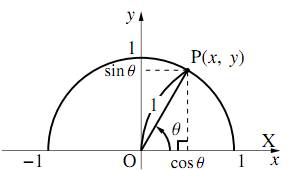
\includegraphics[width=120mm,bb=0 0 287 170]{figures/trigonometry.png}
  \caption{三角比のイメージ図}
\end{figure}

\subsection{三角比の公式}
三角比には, いくつか公式があります. ここを暗記で片づけるのは阿呆のする事です. いったん確認してみましょう.
\begin{eqnarray}
\tan \theta = \frac{\sin\theta}{\cos\theta}
\label{eq:tan}
\end{eqnarray}
\begin{eqnarray}
\sin^2 \theta + \cos^2\theta = 1
\label{eq:square}
\end{eqnarray}
\begin{eqnarray}
\tan^2\theta + 1 = \frac{1}{\cos^2\theta}
\label{eq:tan2}
\end{eqnarray}
式(\ref{eq:tan})については自明ですね. 横の増加量分の縦の増加量なのだから, 傾きです.\\
式(\ref{eq:square})も自明です. ピタゴラスの定理です. 中2でやった. \\
式(\ref{eq:tan2})は一寸ややこしいですが, 式(\ref{eq:square})を用いれば秒で片づけられます. 式(\ref{eq:square})の両辺を $\cos^2\theta$ で割ったのが式(\ref{eq:tan2})です.\\
このように, 三角比の公式というのはおまじないではなく, 常識なのです. 10+20を暗記する人はいませんね?\\
感覚で理解し, すぐにその場で公式を作れるようにしましょう. 



\subsection{三角関数}
さて, 三角比がどんなものか分かったうえで, それぞれの三角比を関数として考えてみます.\\
\\
 $\sin x $はxが$0 + 2\pi n$の時に0, $\frac{\pi}{2} + 2\pi n$の時に1, $\pi + 2\pi n$の時に0, $\frac{3}{2}\pi + 2\pi n$の時に-1を常に通り, その間を滑らかな曲線で結んだ関数になります. n の値は何周目かを表します.\\
\\
$\cos x $も同様にして1 ,0 ,-1 ,0 となっています. \\
\\
$\tan x$ は一寸特殊で, 三角形の斜辺の傾きを表すという性質上, 端がありません. よって x = 0の時には0, で正負方向に対称で$\frac{\pi}{2} + \pi n$で$\infty$ または $-\infty$ を極限としてとんでいきます.\\


ここまでは常識ですね?今時小学生でも知ってるかもしれません.\\
\\
さて, こいつら三角関数の何がすごいかって, 超単純な周期関数である事です. \\
さらに, 実は sin と cos に限って言えば位相が違うだけでその形は全く同じなのです!!!みていてください.\\
\\
\begin{eqnarray}
\cos x = \sin (x + \pi/2)
\end{eqnarray}
こうなっているのです!!やばいですね!!!
\\

\begin{figure}[H]
\label{im:sincos}
  \centering
  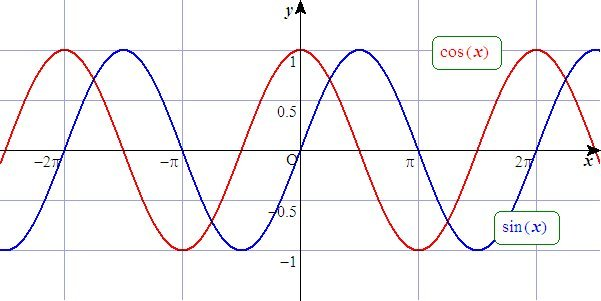
\includegraphics[width=120mm,bb=0 0 601 301]{figures/sincos.jpg}
  \caption{sin / cosの図}
\end{figure}

\subsection{加法定理\label{addition_theorem}}
これはオイラーの公式を用いる事で, 覚えていなくてもその場で導出できます. (オイラーの証明(参照: \ref{euler})) みててください. オイラーの公式より
\begin{eqnarray}
\mathrm{e}^{i(\alpha + \beta)} = \cos (\alpha + \beta) + i\sin (\alpha + \beta)
\label{eq:aplusb}
\end{eqnarray}
指数法則より,
\begin{eqnarray}
\begin{split}
\mathrm{e}^{i(\alpha + \beta)} &= \mathrm{e}^i\alpha + \mathrm{e}^i\beta \\ &= (\cos \alpha + i\sin\alpha)(\cos\beta + i\sin\beta) \\
&= (\cos\alpha\cos\beta - \sin\alpha\sin\beta)\pm i(\sin\alpha\cos\beta + \cos\alpha\sin\beta)
\end{split}
\label{eq:kahou}
\end{eqnarray}
ここで再び式(\ref{eq:aplusb})と見比べると, 式(\ref{eq:kahou})の実部がcos, 虚部がsinの加法になっている事が分かります. ここから三角関数の加法定理は
\begin{eqnarray}
\sin (\alpha + \beta) = (\sin\alpha\cos\beta + \cos\alpha\sin\beta)\\
\cos (\alpha + \beta) = (\cos\alpha\cos\beta - \sin\alpha\sin\beta)
\label{kahouteiri}
\end{eqnarray}

と証明できます. 例のごとくtanは一寸面倒なので, 自分で証明してみてください.
\subsection{正弦と余弦}
sinとcosの関数の定義は分かりましたが, それがなんで嬉しいのでしょうか?\\
これを知るためには, sinとcosの関係はどんなものであるのか考える必要があります.\\
\\
ここで前回やった掛け算が出てきます. \\
任意のsin関数とcos関数の積を考えてみます.\\
\\
$r_1\sin mx $と $r_2\cos nx $です.\\
\\
ここで$r_1$, $r_2$は振幅, mとnは角周波数を示していますので, 異なる周波数の三角関数になっています.\\

\begin{figure}[H]
\label{im:sincos}
  \centering
  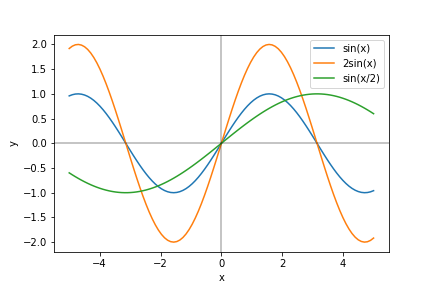
\includegraphics[width=120mm,bb=0 0 432 288]{figures/sines.png}
  \caption{sin / cosの図}
\end{figure}

こいつらの掛け算を考え, さらにそいつを積分してみます.\\
\\
\begin{eqnarray}
  \int^\infty_{-\infty} r_1\sin mx r_2\cos nx dx = \int^{2\pi}_0 r_1\sin mx r_2\cos nx dx = 0
\end{eqnarray}
\\
三角関数は $2\pi$周期で同じ波形の繰り返しになっているので, 範囲が$\infty$ から$-\infty$じゃなくていいのは自明ですね.\\
\\
三角関数は周期関数なので, それぞれが積分すると0なのも自明ですが, 更に積の積分も0になるのです!!!\\
これはすごい!!波としては複雑になっても, 周期関数である事に変わりはなく, 積分しても0になるのは変わらないわけです!!\\
\subsection{関数の内積}
さて, ここで掛け算の復習です. ベクトルの演算, ドット積の定義を覚えていますか?\\
\\
そう, 対応する次元の要素を掛け合わせたものの総和でしたね!\\
\\
これ...関数でも使えそうじゃないですか!?\\
同じxの値の時のy同士をかけ, それの足し合わせをするのもやってる事は同じなのです!!\\
\\
\\
これを使うと, すごい事がおきます. そう. 関数に内積を定義できるのです!!すばらしい!!\\
ただし注意する必要があるのは, ベクトルでは総和をΣで表していましたが, 関数の場合はxが離散値ではなく連続値(参照: \ref{ed})をとるため, 総和はΣでなく∫で表すという事です.\\
\\
いずれにせよ, 掛け算の総和で内積を定義できる事に変わりはないです. これは崇める必要がありそうですね!!\\
\\
たとえば, 
\begin{eqnarray}
f_1(x) = x + 1\\
f_2(x) = 2x 
\end{eqnarray}
という2つの関数を考えてみましょう. 本当は連続値を返しますが, 面倒なのでここではサンプリングレートは整数のみとしましょう.\\
xを1から3で変化させた際のそれぞれの値を算出し, 数列をつくります.
\begin{eqnarray}
{f_1(x=1,2,3)} = {2,3,4}\\
{f_2(x=1,2,3) } = {2,4,6}
\end{eqnarray}
さて, 同じ大きさの数列の, 対応する値同士の積の和でしたね. 求めてみましょう.\\
\begin{eqnarray}
f_1(x)・f_2(x) = \sum_{i=1}^{3} f_1(i)f_2(i) =40
\end{eqnarray}
ドット積がだせました. 関数$f_1(x)$と$f_2(x)$の0から3までのドット積は40でした. これ, 何を表すのかよくわかりませんね. 何回かやってみましょう.\\
\\
0--2, 1--3, 2--4, 3--5, 4--6の範囲でそれぞれ同様の処理をし, $f_3(x)$として並べてみます.\\
\begin{eqnarray}
f_1(0--6) = 1,2,3,4,5,6,7\\
f_2(0--6) = 0,2,4,6,8,10,12\\
f_3(x) = 16,40,76, 124, 184
\label{eq:3}
\end{eqnarray}
この式(\ref{eq:3})はどんな数列になっているでしょう. まず数は$f_1$と$f_2$に比べて$f_3$の時には2つ減ってますね! これはドット積の性質を考えれば明らかで, 3つの数の数列から計算してスカラーを返すわけですから, 両端の点(0と6)の時に計算できなくなるわけです.\\
さらにこいつの変化率ですが, 1項ごとに12xずつ増加していますね!!!\\
\\
元になった$f_1(x)$や$f_2(x)$に比べるとかなり急激な増加をしています. \\
まぁこれも自明ですね, 各区間での元関数の積の足し合わせですからね!\\
\\
つまり, 今回は線形増加する2式だっとのでこうなりましたが, 元関数が不規則な動きをしている場合は, それぞれの性質を平等に反映した新しい関数を作る事ができるわけです!!\\
\\
こいつはバンドパスフィルターなどに使われていて, たとえば速くて細かい挙動をする信号でもゆるやかなカーブを描く低周波関数と掛け合わせることで, 丸くなった新しい関数を定義できるって寸法ですね!!\\
\\
ちょいと雑ですが, 畳み込みとはこの考え方を使って関数をいじいじするやつです!!\\

\begin{figure}[H]
\label{im:convolution}
  \centering
  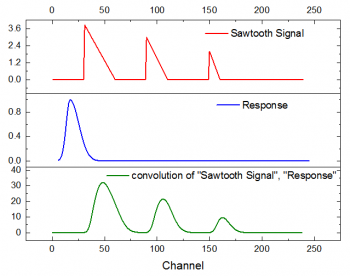
\includegraphics[width=120mm,bb=0 0 350 276]{figures/Convolution.png}
  \caption{畳み込みのイメージ (OriginLabより)}
\end{figure}

\subsection{関数の直行性}
話をもどします. ベクトルにおいて内積が0になるとどうなっていましたか?\\
そう, 直交です!!!\\
\\
ベクトルの内積を関数の内積に拡張する事ができ, ベクトルの内積が0という事は直交を表す...すなわち関数についても直行性を定義する事が出来るのです.\\
\\
sinとcosは直交する関数なんですね!!!すごい!!\\
ここでよくある勘違いについて言及しておくと, 直交と直角は別物です. 留意せよ.
\subsection{直交性}
ここでは関数の直行性については細かい話は省きますが, 直交する関数2つ(sinとcos)を用意できたなら, これを使えばすべての関数を表す事が出来ます.\\
\\
そりゃそうですよねー. 複素数や直交座標系と同じノリです.\\
\\
つまり...全ての(周期)関数は, 異なる振幅, 周波数の三角関数の足し合わせによって表す事ができるのです!!!\\

\begin{figure}[H]
\label{im:furier}
  \centering
  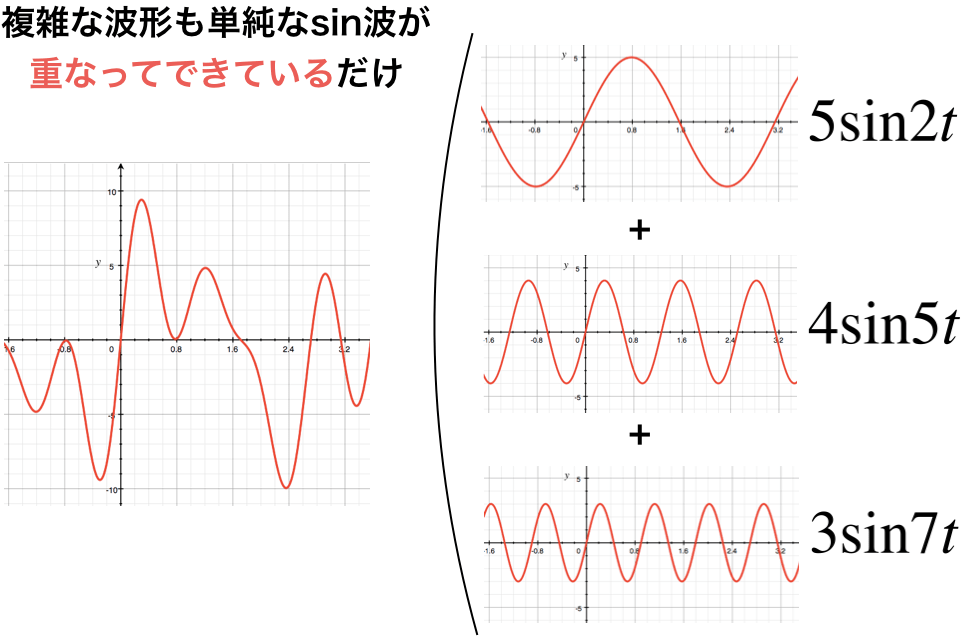
\includegraphics[width=120mm,bb=0 0 974 643]{figures/furier.png}
  \caption{フーリエ変換の気持ち (宇宙一分かりやすいフーリエ変換より)}
\end{figure}

\subsection{フーリエ変換への一歩}
前項での内容を式に表すとこうなります. よく見てください.
\begin{eqnarray}
f(x) = \sum_{n=1}^\infty {a_n \sin(\omega t) + b_n\cos(\omega t)}
\label{eq:sum}
\end{eqnarray}
ここで, 式(\ref{eq:sum})はすべてsin,cosの値が0になる角度の際に吐き出される値も0になるものですが, 実世界においてはそううまくはいかず, DC電源につないでいたらその分基準値が上昇します. そこで式(\ref{eq:sum})を改造します.

\begin{eqnarray}
f(x) = a_0 + \sum_{n=1}^\infty {a_n \sin(nt) + b_n\cos(nt)}
\label{eq:fixed_sum}
\end{eqnarray}

ここで$a_0$はDC電源の分です.\\
\\
脳波は時間によって変化する時間関数ととらえる事が出来るので, この方法で脳波を三角関数に分解して表現する事が出来るのです!!!\\
\\
これが三角関数を崇める理由です.\\
\\
そしてこの, 時間関数f(t)を三角関数の和に変換する事をフーリエ変換といいます. 詳しくは今度.\\
\subsection{大正義オイラーの利用}
とはいえ, 三角関数を$∞$に足し合わせるというのも酷な話で, 計算が面倒なこと面倒なこと...\\
\\
どうにかならんもんか...\\
\\
ん?三角関数の足し合わせ? どこかで聞きましたね?\\
そう, 式(\ref{eq:euler})に表した, 我らが至宝オイラーの公式です!!!\\
\\
オイラーの公式を用いる事で, 三角関数の足し合わせは指数関数で表せます. これを使う事で劇的に計算を楽にする事ができるのです!\\
ただ, オイラーの公式にはsinの前に謎の記号 i がついています. 一体こいつはなんなのでしょう. 次の節では, 虚数と複素数について学びます.\\

\section{複素数}
複素数とは偉大なものであり, 最初は理解に非常に苦しむものです. ですが複素数をマスターするという事は, 整数から分数への拡張や, 正の数から負の数への拡張を遥かにしのぐ恩恵を与えてくれるのです. 高校で習う内容ですが, ここでもう一寸深く学んでみましょう!\\
\subsection{虚数}
虚数の定義からおさらいをしましょう. 高校で習う領域の中でも, 比較的簡単だったはずです.\\
\\
虚数とは, 平方すると-1になる数を基底とした数の事です.\\
\\
1本の直線でしかない実数の問題は, 表現の幅が圧倒的に限られてしまう事です. そこで昔の人類は, 実数軸を2本重ね合わせた直交座標系やベクトルといった考えを用いたわけです.\\
\\
しかし, 虚数の登場がこの常識を大きく変える事になりました!!\\
\\
ベクトルあるいは行列を少し復習しましょう.\\
これらにおいて, 次元はどうやって定義されていたでしょうか? 直交性・独立性ですね!!!\\
\\
実数ではない...0の時以外に必ず実数と交わらず, 直交性をもった「数」を定義できないか?
昔の偉い人はこう考えたのです. 頭おかしいですね!!\\
\\
こうして生まれたのが虚数単位iです. 実数において単位として利用される1の概念と直交する必要があったため, ここで1の平方が1である事に注目しました. \\
\\
平方して負の値になる数は存在しない. これは中学で習う事ですがこれを厳密に言うと, 「従来の数には存在しない」と解釈したわけです.\\
\\
そこで, 平方して負の値になる数を考え, これを虚数と名付けました.\\
実数の単位が1なら, 虚数の単位は1iとなります. 虚数も0の平方にマイナスをつけようとしたところで0なので, 実数と虚数は0で直交する事になります.\\
\\
これが虚数の定義ですね!! 高校数学では「存在しない数」などと習いますがこれは誤解を招きます. 虚数の意義とは「y軸」を定義できる事にこそあるのです!!!\\
存在しない数があったから, 虚数と名付けたのではなく, 実数と直交性を持った数 = 虚数として使えそうな定義はないものかと考えた時に, 平方すると -1 になる数, を考え付いたわけです.

\subsection{虚数の性質}
虚数は単位iがついてるだけなので, 基本的な足し算引き算はすべて実数と同様に扱えます. 簡単ですね!\\
\begin{eqnarray}
3i + 5i  =(3 + 5)i = 8i
\end{eqnarray}
掛け算になると一寸難しくなり, 虚数同士をかけると数字同士の積にマイナスをつける必要があります. それが虚数の性質でしたね!\\
\begin{eqnarray}
3i * 5i = (3*5)i^2 = 15 * -1 = -15
\end{eqnarray}
\\
この掛け算, 実は複素数の掛け算の性質を考えると自明になります.\\
この章の最後でそれを説明します!\\
\subsection{複素数}
虚数のおさらいができたところで, 複素数です. 実数も虚数も直線であるため, これらを軸として, 直交座標系っぽいものを考えます.\\
\\
こうしてできた平面の事を, 複素平面やガウス平面といいます.\\
\\
さて, ガウス平面を考えた際, とてもうれしい事が数多くあります. まずはそれぞれの軸における長さですが, 実数も虚数も単位が1(i)であるため, 原点からの距離を考えると $ |x| = |xi| $ になっているのです. \\
\\
この性質を利用すると, ガウス平面上の任意の点を直交座標の点に対応づける事ができ, (x, y) ≒ x + yi といった具合に表す事が出来ます. \\
\\
このように, 実数部分と虚数部分の足し合わせによって, 複素平面(二次元)上の数を表現した数を複素数といいます.\\
\\
こいつのうれしさは, 直交座標や行列のように複数の数の集まりではなく, ひとつの数として扱える点です!!!\\

\begin{figure}[H]
\label{im:imagine}
  \centering
  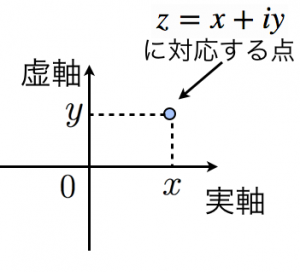
\includegraphics[width=100mm,bb=0 0 300 272]{figures/gauss.png}
  \caption{虚数軸 (高校数学の美しい物語より)}
\end{figure}

\subsection{数の大幅な拡張}
複素数の定義が分かったところで, これが実際にどうやって影響してくるのかについて考えます. 一次元が二次元に拡張されたわけですからその恩恵は計り知れません. \\
\\
さらに複素数の偉大な点は, 実数を複素数の一部として扱える点です.\\
\\
たとえば3は, 複素数で表すと 3 + 0iとなります.\\
そして注意しないといけないのは, 複素数を実数に変換した場合, その虚数成分は捨てられてしまうのです!!\\
実軸に投射される過程で, 虚軸(高さ)成分は消えてしまうという事です.\\
\\
つまり...\\
我々が今まで3だと思ってた数は, 実は 3 + 5i かもしれない...という考え方もできます!!\\
\\
ちょっと違うような気もしますが, たとえば大学の単位で考えましょう.\\
成績がCでもSでも, 来る単位は1です.\\
\\
実軸を単位, 虚軸を成績とすると, 実軸だけではCの人もSの人も同じ優秀さぽく見えますが, 虚数成分も合わせれば同じ単位取得者でも上下関係があった事に気付けるわけです!!\\
\\
複素数は偉大ですね!!
\\
実はこの考え方が後にウェーブレット変換を学ぶ際に非常に重要になるのです. 頭の片隅においておいてください.\\

\subsection{複素数平面}
複素数平面において, 任意の点 x + yi を表す方法について考えていきます. \\
\\
実軸と虚軸の直行性より, 複素数 z = x + yi の横(実部Re)の長さ(\ref{eq:x})と, 縦(虚部Im)の長さ(\ref{eq:y}), 原点との距離(\ref{eq:length}), そして実軸との間になす角(\ref{eq:arg})はそれぞれ
\begin{eqnarray}
\mathstrut Re z = x
\label{eq:x}
\\
\mathstrut Im z = y
\label{eq:y}
\\
|z| = \sqrt{x^2 + y^2}
\label{eq:length}\\
\mathstrut arg z = \tan^{-1} \frac{y}{x}
\label{eq:arg}
\end{eqnarray}
のように表されます. 長さについては直交座標なので自明ですね. 絶対値に関してもピタゴラスの定理より自明. 式(\ref{eq:arg})で表される角の事は, 偏角と言います. 実軸との角度の事であるので, tanを使って表す事が出来るというわけですね.\\
\\
また, 複素数 z を実軸に線対称な点を取った点の事を $ \overline{z}$ と表し, 複素共役な点といいます.\\

\begin{eqnarray}
z = x + yi
\end{eqnarray}
\begin{eqnarray}
\overline{z} = x - yi
\end{eqnarray}

\begin{figure}[H]
\label{im:complex}
  \centering
  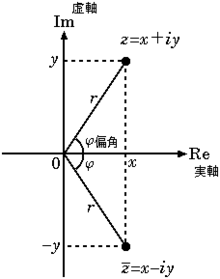
\includegraphics[width=100mm,bb=0 0 220 279]{figures/Complex.png}
  \caption{複素平面 (wikipediaより)}
\end{figure}

\subsection{極形式}
複素数 z は x + yi のような表記の仕方以外に, もう一つの表し方ができます.\\
\\
前節で確認した, 複素数 z の絶対値は, 原点との距離を表す実数でした. 範囲は0以上の実数になりますね!!\\
\\
偏角の取りうる範囲はどうなるでしょうか?\\
原点を中心として4つの象限をぐるぐる回るので, -π ~ πですね!\\
\\
\\
この2つに注目して考えます. 原点からの距離(r)と偏角($\varphi$)が分かるという事は, 平面上で一意に定まる点を定義できますよね?
\begin{eqnarray}
z = x + iy = r(\cos \varphi + i\sin \varphi)
\label{eq:kyoku}
\end{eqnarray}

$r\sin\varphi$ で導出される数は実数(y)になっているため i をかける事を忘れないように.\\

\begin{figure}[H]
\label{im:polar}
  \centering
  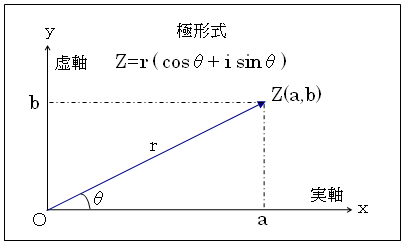
\includegraphics[width=120mm,bb=0 0 406 246]{figures/polar.png}
  \caption{極形式 (はてなフォトライフより)}
\end{figure}

\subsection{大正義オイラー再び}
式(\ref{eq:kyoku})の最右辺をよく見てください. どこかで見た式ですね!!!\\
人類の至宝を利用する事により式(\ref{eq:kyoku})はこのように変換する事が出来ます.\\
\begin{eqnarray}
z = x + iy = r(\cos\varphi + i\sin \varphi) = r \mathrm{e}^{i\varphi}
\end{eqnarray}

\subsection{複素数の掛け算}
さて, 複素数を $r\mathrm{e}^{i\varphi}$ で表せたところで, 何度か説明をしている複素数の掛け算を改めて考えます.\\
\begin{eqnarray}
\begin{split}
z_1 * z_2 = (x_1 + iy_1)(x_2 + iy_2)\\
&= r_1(\cos\theta_1 + i\sin\theta_1)r_2(\cos\theta_2 + i\sin\theta_2)\\
&= r_1r_2\mathrm{e}^{i\theta_1} \mathrm{e}^{i\theta_2}\\
&= r_1r_2\mathrm{e}^{i(\theta_1 + \theta_2)}
\end{split}
\end{eqnarray}

こうなっているのです!!!\\
複素数の掛け算は絶対値をかけた上の回転を表すのですね!!
\subsection{戻り学習}
ここで再び, 虚数とは何か, 何故平方すると-1になるのかを考えます.\\
任意の複素数を考えます. ここでは面倒なので $ 3 + 0i$ としましょうか.
\begin{eqnarray}
3 + 0i = 3(\cos 0 + i\sin 0) = 3(1 + 0) = 3
\end{eqnarray}
こんな感じに表せますね.\\
こいつにiをかけます. よく見ててください.
\begin{eqnarray}
i(3 + 0i) = 3i(\cos 0 + i\sin 0) = 3i(1+0) = 3i\\
\end{eqnarray}
そしてこいつと...
\begin{eqnarray}
3(\cos (0+\frac{\pi}{2}) + i\sin (0 + \frac{\pi}{2})) = 3(\cos\frac{\pi}{2} + i\sin\frac{\pi}{2}) = 3i
\label{eq:roll}
\end{eqnarray}
こいつを見比べるのです. 同じ値になってますね!!\\
複素数の積は回転を表すので, つまり i をかけるという事は $\frac{\pi}{2}$ 回転するという事なのです!!\\
\\
なのでもちろん式(\ref{eq:roll})にiをかけると, -3 になります. 虚数単位i を2回かけると-1を掛ける事になる, つまり $\pi$ 回転するのですね!\\
\subsection{まとめ}
このように三角関数と虚数は非常に親和性が高く, そしてオイラーの公式によって指数関数ともつながる非常に重要な概念になっています. \\
\\
三角関数と虚数を理解すれば, 脳波解析を学ぶ基礎となる数学はほぼ出そろったという事になります!!\\
しっかりと理解していってください!!\\

\section{微分・積分}
この章ではみんな大好き微分積分いい気分の気持ちを考えていきます.\\
高校数学で習うなかでも, とびっきり意味が分からない分野ですね.\\
\subsection{極限とは}
まず, 微分や積分といった計算は超極小の範囲で考える数学です. この超極小というのがなんなのかから考えます.\\
\\
超極小...曖昧な響きですね. 我々の身長の話をしている際にmmを持ってきたら極小と言えますが, 蟻の体長の話をしている時には大きすぎますね. \\
\\
このように, どんなスケールでの話をしていても十分に小さいといえるようなスケールでの話が微分積分です.\\
\\
実用では「0に限りなく近づく」などといった表現で表され, 数式だとこうなります.
\begin{eqnarray}
\lim_{x\to0} f(x)
\end{eqnarray}
この意味するところは, 関数f(x)のxを限りなく0に近付けた時の関数の返す値という事になります. つまり f(x) が 2x とかであれば
\begin{eqnarray}
\lim_{x\to0} 2x ≒ 0
\end{eqnarray}
になります. しかしここでxは限りなく0に近い値なので実質的にはこの式が返す値も0と見做せるので, 等号は成り立ち, 点々は外れます.
\begin{eqnarray}
\lim_{x\to0} 2x = 0\\
\lim_{z\to\infty} 2x = \infty
\end{eqnarray}
\subsection{ε-δ論法 \label{ed}}
限りなく0に近いって曖昧な表現ですよね. さっきも言ったようにmmなのかμmなのか, どこからが限りないと言っていいのかわかりません. ここで極限
\begin{eqnarray}
\lim_{x\to a} f(x) = b
\end{eqnarray}
は数学語では
\begin{eqnarray}
\forall \varepsilon >0, \exists \delta>0  s.t.  \forall x \in \mathbb{R}, |x-a|<\delta \Rightarrow |f(x)-f(a)|<\varepsilon
\label{eq:ed}
\end{eqnarray}
のように定義されます. 有名なε-δ論法というやつを使うのです.\\
\\
この式の意味はこうです.\\
\\
「任意の正の数εに対し, ある適当な正の数δが存在し, $ 0 < |x − a| < δ$ を満たす全ての実数 xに対し、 $|f(x) − b| < ε$が成り立つ」\\
\\
f(x)とbの間の距離が任意の正の数εより狭い範囲において, 必ず対応するxの値が存在しているといった具合で, 「お前がどんなに頑張ろうと俺はその上をいく」みたいなやつです. これが連続値の定義になるわけですね.

\begin{figure}[H]
\label{im:ed}
  \centering
  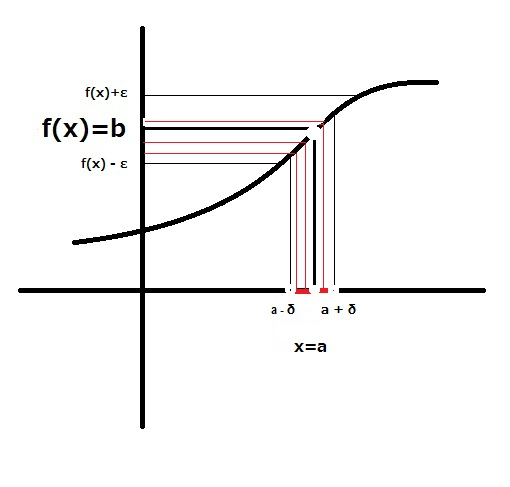
\includegraphics[width=120mm,bb=0 0 510 487]{figures/ed.jpg}
  \caption{ε-δ論法. aの左側は連続だが右は連続じゃない}
\end{figure}

つまり極限とはmmなのかμmなのか?という問いに対する答えは, 「お前がmの話をするならcm, cmの話をするならmm, mmの話をするなら...」を死ぬまでやるイタチごっこだということです!!\\
\\
ちなみに式(\ref{eq:ed})はついでに関数の連続性についても定義していて, どんなに小さい範囲で見てもそれより小さい値が存在するという事は切れ目なくしっかりとつながっている=連続であるという定義にもなります.\\

\subsection{微小な変化率}
さて, 極限とはある一点に限りなく小さい範囲を考える事でした.\\
ここで, 関数でも同じ事を考えます.\\
\\
まずはざっくりとした範囲で考えてみましょう.\\
\begin{eqnarray}
\lim_{0\to5} x = 5
\end{eqnarray}
この式の意味を考えてみます. 「xの値が0 から5に限りなく近づくとき, yの値は何になっていくか」ですね!\\
\\
ぶっちゃけて言えばxが5増えたらyはどんだけ増える?という問いで, それに対する答えが「5」だったわけです.\\
\\
変化する値が2つあったら, その間の比を求めたくなるのが健常な脳の持ち主です. xが増えた分に対してyがどれだけ増えたかを考えましょう.
\begin{eqnarray}
\frac{\Delta y}{\Delta x} = \frac{5}{5} = 1
\end{eqnarray}
こうですね. Δは増加分という意味です.\\
これ, あれですよね. 中学で習った変化の割合, またの名を平均変化率, またの名を傾きでした.\\
今回は傾き1の一次関数を例にしたので, 変化の割合もしっかり1になっています.\\
しかしこれが二次以上の関数だった場合どうなるでしょう? 元が直線でないので, 重なる事はないはずです.\\
\begin{eqnarray}
\lim_{x \to a} f(x)
\end{eqnarray}
このうち, f(x)が二次以上の関数の場合は $|x-a|$の値が大きければ大きい程グラフの形を無視して串刺しにする線が引かれ, 小さい程グラフの縁の角度に近い線が引かれていきます.\\

そしてこの値が一点に集中したとき, つまり$|x-a|$が0となったとき, それは点aにおける接線の式になるのでした.\\
\\
これはつまり, 超微小で見た変化率=接線を求めているという事で, この操作をする事を微分と言います.\\
\\
微分とは, 局所的な微小変化率を求める事なのです!!!\\
「あたりまえだろお前高校数学やったか?」と思っただろ!!やってねえんだよ!!\\
\\
実際この微分の捉え方, よく理解できている人は多くないように思えます. かみしめてください.

\begin{figure}[H]
\label{im:sessen}
  \centering
  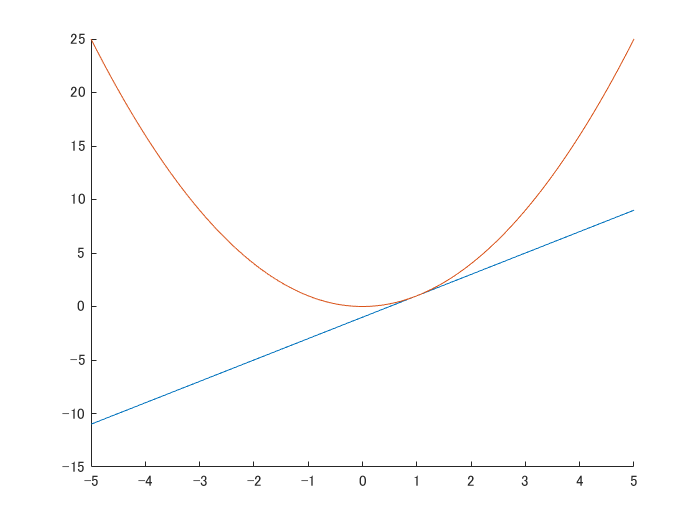
\includegraphics[width=120mm,bb=0 0 700 525]{figures/sessen.png}
  \caption{局所的な微小変化率 = 接線}
\end{figure}

\subsection{三角関数の微分}
上記の性質が分かっていれば, 簡単な公式達です. 覚えるまでもありません.
\begin{eqnarray}
(\sin x)' = \cos x \\
(\cos x)' = -\sin x \\
(-\sin x)' = -\cos x \\
(-\cos x)' = \sin x
\end{eqnarray}
\\
自明ですね. sin, cos関数それぞれがどういった挙動をしていて, その傾きをすべての点で取ってつなげていったらどうなるかを考えれば, 自ずと分かるはずです.\\
\\
「微分とは, 局所的な微小変化率を求める事」です.\\
\subsection{ネイピア数}
三角関数の次, 微分といったらこいつですよね. πと並び超越数として名高い e の出番です.\\
ネイピア数は別名オイラー数です. これだけで崇めないといけない気がしてきますね!?\\
\\
$(\mathrm{e}^x)' = \mathrm{e}^x$ つまり, 指数関数にしたときに微分しても値が変わらないという変態な数です.\\
\\
微分しても値が変わらないって, わけがわからないですよね. 微分とは傾きを求める事だとか, 体積から面積を求める事, といった理解をしていると全く訳がわからなくなります.\\
\begin{eqnarray}
e = \lim_{x\to 0} (1+x)^\frac{1}{x} = \lim_{x \to \infty} (1+\frac{1}{x})^x
\end{eqnarray}
定義としてはこんな感じです.\\
まぁここは良いです. 大事なのは指数関数を微分しても値が変わらないという性質の確認だけです.\\
\\
さて, 一般に正の1以上の数を底とする指数関数は, 第一象限で二次関数的な上がり方をし, (0,1)を通って, 第二象限ではx軸に漸近しつつ徐々に横ばいな形をとりますね?\\
\begin{figure}[H]
\label{im:sisuu}
  \centering
  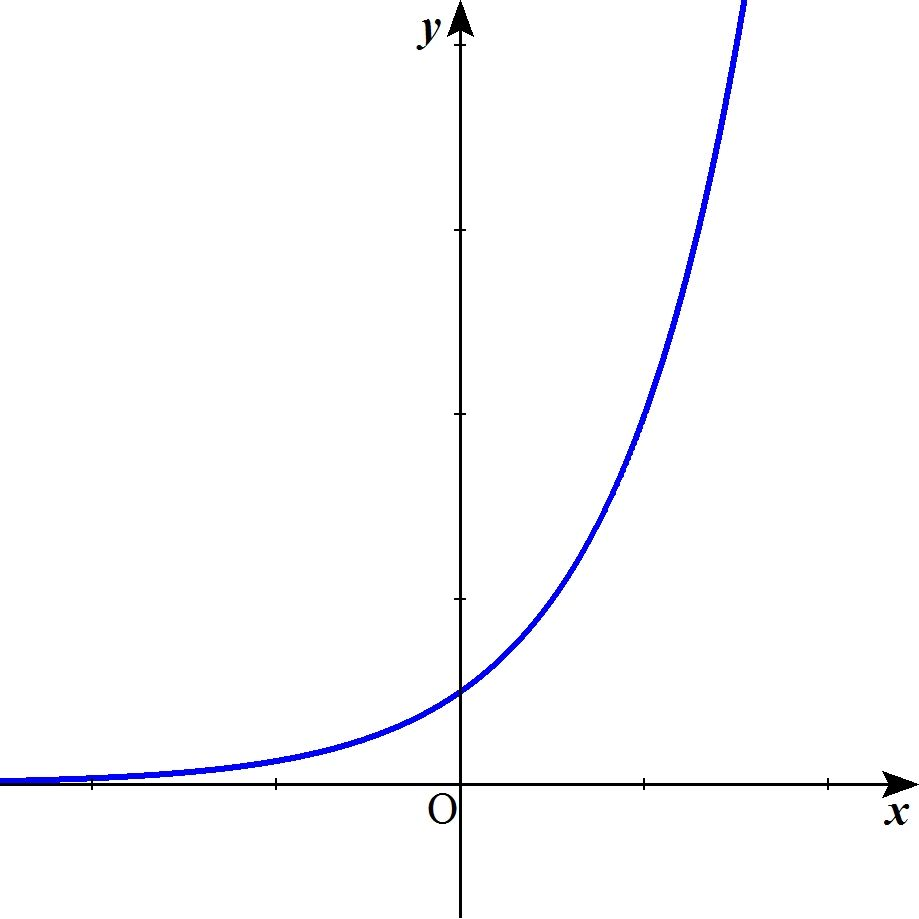
\includegraphics[width=120mm,bb=0 0 919 919]{figures/sisuu.jpg}
  \caption{指数関数}
\end{figure}

こいつを, x軸方向に様々な点で接線ぽいのを引き, 傾きを推測してみてください. \\
\\
面白い事に, こうやって求めた傾きの値をy成分として新しくグラフを書いた f(x)' も指数関数の形をしているのです!!\\
そしてこの形は, (0,1)だけは固定としてその開き方が底の値によって異なります. \\
底の値次第で, 微分したら開いた指数関数がでてくるものや, 細くなった指数関数がでてくるのです.\\
\\
もう分かりますね?ネイピア数とは, 丁度この開いたり閉じたりする境界にある数なのです!!\\
よって微分しても出てくる指数関数は開き具合を変えず, 重なった関数となるのです.\\
\\
ネイピア数の何がすごいかって?\\
いろんな数学に利用できるところです!!!\\
\begin{eqnarray}
\mathrm{e}^{i\theta} = \cos\theta + i\sin\theta \\
F(x)=\frac{1}{\sqrt{2\pi \sigma^2}}\int_{-\infty}^{\infty}\exp{\left\{-\frac{(x-\mu)^2}{2\sigma^2}\right\}}\ \mathrm{d}x
\end{eqnarray}
書くのが面倒なのでいかついのは1個だけにします. ガウス関数ですね. 統計とか信号処理やるときにでてきます. 上は言わずもがなのオイラーの公式です.\\
\subsection{積分}
さて, 微分がわかったとこで積分の気持ちです. パパっといきます.\\
まず, 計算の上でいえる事としては, 微分の逆の操作をするという事です.
\begin{eqnarray}
\int 2x dx= x^2 + C
\end{eqnarray}
こんな具合でしたね. \\
微分とは微小な増分であるdxとdyを用いて変化率を求めるものでしたが, 積分の場合は, dxとyを用いて面積を求める操作になります.\\
\\
関数f(x)は x = a の時, f(a)という値を取り, x = b の時, f(b)という値を取ります. この時xの増分 dx は, x軸での距離を表すので横の長さととらえる事ができ, f(a)あるいはf(b)は縦の長さと考える事ができます.\\
\\
こうして定義される横と縦を用いて作られる長方形を, a~b, b~c, c~d..., m~nといった範囲で同じように作っていき, それぞれの面積をたすと, 関数f(x)とx軸の間の, a~nにおける面積っぽいものがだせますね!\\
しかしこのとき, 横はまだしも縦の長さが問題です. 左端に合わせるのか右端に合わせるのか, あるいはその中点にするのか... これによって求められる面積は理論値から離れた値になってしまいます.\\
\\
この問題を解決するにはどうしたらよいでしょうか?\\
簡単ですね, x軸上での幅を限りなく小さくしていけばよいのです!!\\
\\
横幅が限りなく0に近づいた時, 左端と右端のとる高さは同じ値となるため, 微小長方形の形も関数f(x)にそったものになるはずです.\\
\\
そしてそれらを足し合わせれば, デコボコではなく滑らかな, 関数f(x)の凹凸にあった面積を導出する事が出来るのです!!!
\begin{eqnarray}
\int_a^b f(x) dx
\end{eqnarray}
とはつまり...\\
xがaからbの範囲において, それぞれの f(x) = 高さと 微小なdx = 幅をかけたもの = 面積を足し合わせる\\
といった意味になっているのです!!!

\begin{figure}[H]
\label{im:integral}
  \centering
  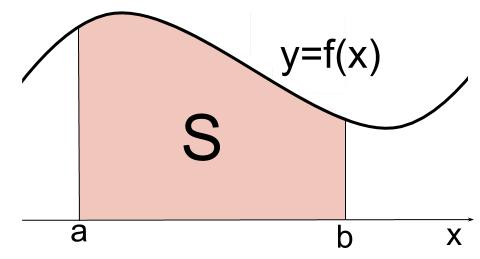
\includegraphics[width=120mm,bb=0 0 480 259]{figures/int.jpg}
  \caption{積分と面積の関係}
\end{figure}
\subsubsection{足し算としての積分}
積分とは微小面積の足し合わせと言いましたが, 足し算はΣで表されたはずです. 何故∫を使うのでしょうか?\\
\\
答え. Σは離散値の計算にしか使えないからです!\\
\begin{eqnarray}
\sum_{k=1}^{n} k
\end{eqnarray}
この式では, kに入る数字は1からnまでの整数になります. 無限小の幅による微小面積を考えるときにこれでは, 全く意味がないですよね.\\
\\
そこで∫を使うと, 整数に限らずすべての数を足し合わせる事が出来るのです!!\\
素晴らしいですね!!!足し算のアップデートです!!!\\
\\
足し算として積分を使うことは, ここからの数学では, 頻繁に出てくるので是非感覚として理解してください.
\begin{eqnarray}
X(f) &=& \mathcal{F}[x(t)] = \int^{\infty}_{-\infty}x(t)\exp(-j2\pi f)dt \\
 x(t) &=& \mathcal{F}^{-1}[X(f)] = \int^{\infty}_{-\infty}X(f)\exp(j2\pi f)dt 
\end{eqnarray}
たとえばこいつらは複素フーリエ変換とその逆変換の式ですが, これらもx(t)とexpなんたらの掛け算の-∞から∞での総和とかのように解釈する事ができるわけです!!!\\
これが積分を学ぶ意味です.

\section{統計学}
\subsection{基本統計量}
この節では統計の基礎を学びます. 統計は脳波解析に直接的に使うわけではありませんが, 解析した結果がいいデータなのかゴミデータなのかを判断したりするために必要です. また, 分野問わずどんな論文も統計の知識なくては読むことが出来ません. 幾何学などに比べれば大した事ない量とレベルなので, パパっと身に着けちゃいましょう!! (脳にフィットするとは言っていない)\\
\\
さて, まずは冗談じゃなく小学生でも知ってる統計学から始めましょう.\\

\begin{figure}[H]
\label{im:histgram}
  \centering
  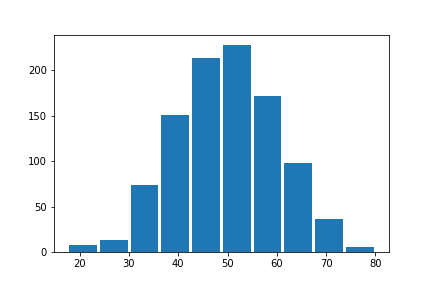
\includegraphics[width=120mm,bb=0 0 432 288]{figures/hist.png}
  \caption{平均50, 標準偏差10の1000個のランダムデータ}
\end{figure}

複数の数値データ$x_i = [x_1, x_2, x_3, ...]$が得られた際, とりあえず平均と分散, ついで標準偏差を求めたくなるのは類人猿の性ですね.\\
\begin{eqnarray}
\label{eq:ave}
\bar{x} = \frac{\sum_{i=1}^{n} x_i}{n}
\end{eqnarray}

\begin{eqnarray}
\label{eq:var}
s^2 = \frac{\sum_{i=1}^{n} (x_i - \bar{x})^2}{n}
\end{eqnarray}

\begin{eqnarray}
\label{eq:dev}
s = \sqrt{s^2} = \sqrt{\frac{\sum_{i=1}^{n} (x_i - \bar{x})^2}{n}}
\end{eqnarray}

とりあえず, 平均(\ref{eq:ave})と分散(\ref{eq:var}), 標準偏差(\ref{eq:dev})の式を書いてみました. 平均は良いですね?全要素を足して要素数で割るだけです.\\
分散は, 一見ややこしくなってるかもしれませんが各要素と平均の差(偏差)を足して, 同じく要素数で割っています. 標準偏差はその平方根です.\\
\\
平均とは, 得られたデータのだいたい「真ん中あたり」を指す指標です. 代表値として, 他には中央値とか最頻値とかがいますが, まあ平均値だけ覚えていれば大丈夫です. モブは放置.\\
\\
分散とは, 偏差の平均ですね?つまり, 得られたデータはどれだけ平均付近に固まっているか, あるいはバラバラになっているかを指します. 各要素が平均から遠い値であるほど, 偏差とその二乗は大きな値を取ります. 2乗するのは, 符号の影響をなくすためです. そいつらの平均なので, やはり値が大きい程データがばらついているという事になります.\\
\\
標準偏差は, 分散の平方根です. それだけ. 偏差の特性上, 分散を導出する際にデータを2乗してしまっているため, 分散は元のデータとスケールが違います. 例えば元データが長さだったら, 分散は面積を表してしまいます. なので平方根をとって次元をそろえてあげるわけですね. これで分かりやすくなります.\\
\\
図(\ref{im:histgram})に設定した統計量とヒストグラムを見比べて, 感覚を確認してください.
\\
こいつらは後程アップデートされたりしますが, 基本的にはデータを扱う上で普遍的に利用されるものです. まず確実に理解しておきましょう.\\
\\

\subsubsection{正規化}
ちなみに, 標準偏差と平均をどう使ってデータを読み解くのかという例として, こんなのもあります.

\begin{eqnarray}
z_i = \frac{x_i - \bar{x}}{s}
\end{eqnarray}

正規化(標準化)と言われる処理です. 各要素と平均との偏差を標準偏差で割っていますね. 標準偏差はざっくり言うなら偏差の平均的なやつですので, それと各偏差の比を見ているわけです. こうする事で, 平均0, 分散1のデータに置き換える事が出来るので, それぞれの要素がどれくらい平均から外れているかが分かりやすくなります. zの大きさが1を超えれば平均からかなり(正なら正方向, 負なら負方向に)離れているってわけですね!!\\

\begin{figure}[H]
\label{im:z-hist}
  \centering
  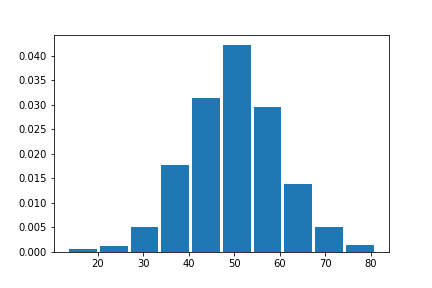
\includegraphics[width=120mm,bb=0 0 432 288]{figures/z-hist.png}
  \caption{正規化した, 同じ条件の図(\ref{im:histgram}}
\end{figure}

まぁ, 勿論こんな事しないでそのまま眺めるだけでも十分だったりしますが.

\subsection{相関と共分散}
次もよくつかわれる基礎です. 2つ以上の変数を持つデータ(たとえばAさん,Bさん ... の身長と体重)の性質を検証する術です. \\
\subsubsection{相関と散布図}
相関は非常に簡単です. 直交座標軸横軸に変数1, 縦軸に変数2をおいて, あとは得られたデータをすべて対応する位置にデータを点でプロットしていくだけです. こうして得られた, 点を散りばめられた図を散布図だとか相関図と言います.\\
この図の特徴ですが, データによって点の散らばり方が変わります. たとえば先程の身長と体重の例の場合, 一般的に身長が高い人の方が体重が重い傾向にありますね?これは図では点が右肩上がりの斜めライン付近に多く集まる事を意味します. \\
逆に, 右肩上がりの斜めに点が集まるという事は, 一方が上がると他方も上がる, 比例に似た関係にあると言えます. 逆に右肩下がりの場合, 一方が上がると他方が下がる関係ですね!!\\

\begin{figure}[H]
\label{im:scatter1}
  \centering
  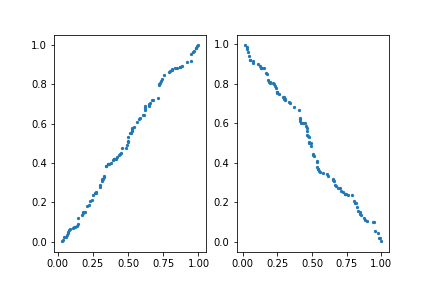
\includegraphics[width=120mm,bb=0 0 432 288]{figures/scatter1.png}
  \caption{左: 正の相関図 右: 負の相関図}
\end{figure}

\begin{figure}[H]
\label{im:scatter2}
  \centering
  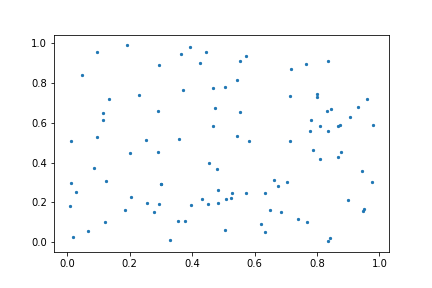
\includegraphics[width=120mm,bb=0 0 432 288]{figures/scatter2.png}
  \caption{相関なし}
\end{figure}

前者を正の相関, 後者を負の相関があるといいます.散布図を描いた時の見た目でなんとなくデータ間の関係が分かるわけです. 見た目ではっきり分かるほど点が線状に並ぶ程, 相関が強いと表現されます(図\ref{im:scatter1} はかなり強い). 逆に見た目で何も分からん場合(図\ref{im:scatter2})は, データ間には相関がないと言えます. \\
非常に便利なので, アンケートデータとか取ったらとりあえずプロットしてみると良いです. 低レベルな卒論だとこれだけやって出していたりも...?\\
\\
\subsubsection{回帰}
ちなみにですが, 今は相関を見る際になんとなくで評価しましたが, それっぽい位置に線を引いてあげる (回帰) とよりデータの傾向を強く感じる事が出来るはずです. この, 「それっぽい線」というのが実は曲者で, ひとまず目算でも良いのですが正確に書く場合, メジャーな方法では最小二乗法などが使われます. \\
そう, 近年では意識スカイツリー系イケイケ起業マンたちに「AI」と呼ばれていたりもするあれです!!!散布図が描けて, あとは最小二乗法(図\ref{im:predict})が使えちゃえばAIエンジニアが名乗れるのです!!!素晴らしいですね!!\\

\begin{figure}[H]
\label{im:predict}
  \centering
  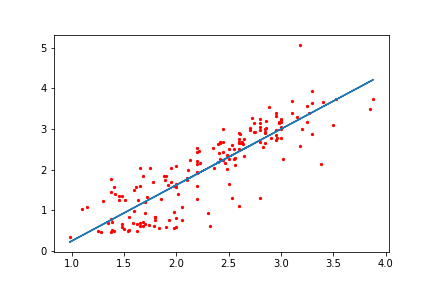
\includegraphics[width=120mm,bb=0 0 432 288]{figures/predict.png}
  \caption{AIエンジニアわい迫真の単回帰分析}
\end{figure}

\subsubsection{共分散}
変数間の関係を探るのに非常に便利な相関ですが, やや客観性にかけていた事に気付くでしょう. 「なんとなく」「それっぽい」などの語彙を多用していたはずです. これでは困ってしまいますので, より客観的に評価する方法を考えます.\\
\\
それが共分散というやつで, 普通の分散は1変数において偏差の二乗平均を取るわけですが, 共分散では2変数の偏差同士を掛け合わせます. こうする事で, それぞれの偏差の特徴を反映させた新しい分散を定義する事が出来ます. \\
\\
それぞれの特徴とは, 偏差の符号です. 1変数分散の場合は単に二乗してしまうため符号は外れますが, 共分散の場合はそれぞれの偏差の符号が異なった場合には負の値を取ります. 偏差の符号が異なるというのは負の相関が, 同じなら正の相関があるという事です.\\
さらに, 絶対値の方も有用な情報をくれます. それぞれの偏差が大きい程, 共分散の絶対値も大きくなるわけです. これは相関の強さを表します.\\

\begin{figure}[H]
\label{im:co-var}
  \centering
  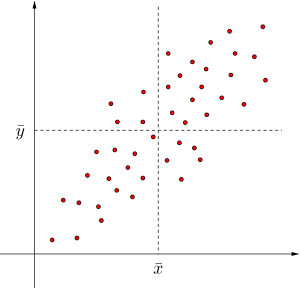
\includegraphics[width=120mm,bb=0 0 432 288]{figures/kyoubunnsann.png}
  \caption{適当な散布図. どの象限に点が多いかで共分散の値が決まる(高校数学の美しい物語より)}
\end{figure}

この2つを合わせる事で, 共分散は次のような性質を持ちます.\\
\\
共分散は$S_xy$, 変数xと変数yの相関が強い程絶対値が大きくなり, その符号は相関の正負に一致する.
\\
式は以下です.\\
\begin{eqnarray}
\label{eq:covar}
S_{xy} = \frac{\sum_{i=1}^{n} (x_i - \bar{x})(y_i - \bar{y})}{n}
\end{eqnarray}

\subsubsection{相関係数}
ただ, 共分散は分散と違い, かけている変数の単位が違うため, 数字自体に意味はない事に注意が必要です. 例えばmmとmgで算出したときと, kmとkgで算出したときとでは同じデータなのに共分散の値が大きく変わってしまいますし, 単純に平方根を取ったところで違う単位系の積になってるので読み取れる情報がありません.\\
\\
そこで, 共分散版の標準偏差的なものを定義してあげます. それが相関係数です.\\

\begin{eqnarray}
r_{xy} = \frac{S_{xy}}{S_x S_y} = \frac{\frac{\sum_{i=1}^{n} (x_i - \bar{x})(y_i - \bar{y})}{n}}{\sqrt{\frac{\sum_{i=1}^{n} (x_i - \bar{x})^2}{n}} \sqrt{\frac{\sum_{i=1}^{n} (y_i - \bar{y})^2}{n}}}
\end{eqnarray}

分子が共分散になっているので, 分母にはそれぞれの標準偏差を入れているのですね. これにより相関係数はその単位に関係ない評価が出来るようになります. 当然, 共分散が標準偏差同士をかけたやつよりも上回る事はないので, 相関係数は -1から1の間の値を取ります.\\
相関係数の値が-1に近い程負の相関が強く, 1に近い程正の相関が強いわけですね!!!便利です!!\\











\chapter{応用数学}
さて, 基礎を学んだところで, ここからはいよいよ理工系の学生, 脳というブラックボックスに挑む学生として学ぶべき, 高度な数学に挑戦していきます.\\ 
わくわくしますね!!!\\
\section{オイラーの公式 \label{euler}}
まずはオイラーの公式の導出からいきましょう!!!\\
\\
今まで, 証明をずっと後回しにしてたくせによく使っていた理由は, まずこの公式の導出には様々な数学的知識が必要であることです. また, やや直感的に分かりにくい公式であるため, 導出より先にその利便性, 利用のされかたに触れて慣れてほしかったのです.\\

\subsection{オイラーの公式を翻訳する}
改めて, オイラーの公式を眺めてみましょう.\\
\begin{eqnarray}
\mathrm{e}^{i\theta} = \cos x + i\sin y
\end{eqnarray}
うーん, 美しいですね.\\
\\
こいつをちょっと解剖してみましょう. 数学語を日本語に翻訳すると, おそらくこんな感じになります.
\\
\\
底をネイピア数eとし, 指数関数 $\mathrm{e}^x$のxに角度Θを代入し, 虚数単位iをかけたもの(左辺)が, sin と cos の足し算で表した何らかの値と同じ値を表している.\\
\\
うーん謎ですね.\\
なぜ指数関数が三角関数で表せるのか?\\
三角関数の足し合わせってなんだよ?\\
指数関数を虚数にするってなんだよ??\\
\\
\\
私はここで脳がオーバーヒートを起こし, 拒絶反応を起こしたものです.\\
\\
指数関数が三角関数で表せるのは, オイラーの公式が成り立つ事が分かったからだ. つまりは結果論でとらえていいでしょう.(いやまぁ, 本当は違うけども) \\
三角関数の足し合わせとは, 複素数の事だ!!(つまり cos と isin です)\\
\\
どうしても分からないのは無視しよう!!!\\
\\
というのも, オイラーの公式は偶然発見されたと考えた方が気が楽になるのです. 厳密に理解するのは難しい.\\
\\
\\
理解が進めば, おのずと脳に適用されます.
\subsection{マクローリン展開}
さて, 一旦オイラーの公式は忘れてみましょう.\\
\\
大学で学ぶ数学, とりわけ微分積分において最初に我々が躓く単元に, テイラー展開・マクローリン展開がありますね!\\
\\
オイラーの公式は, このマクローリン展開さえ分かれば一瞬で導出する事が可能です.\\
\\
テイラー展開とマクローリン展開の違いは, テイラー展開の限定された特殊形がマクローリン展開です. なのでマクローリン展開だけここでは扱います.\\
\begin{eqnarray}
f(x) = \sum_{k=0}^\infty f^{(k)} (0) \frac{x^k}{k!} = f(0) + f'(0)x + \frac{f''(0)}{2!}x^2 + \frac{f'''(0)}{3!}x^3 ...
\end{eqnarray}

これがマクローリン展開です.\\
元関数f(x)を多項式で近似するわけですね.\\
\\
そしてここで使われる多項式が, fのx=0の時の高階微分係数から定まっているわけです!!!\\
\\
こいつの凄いのは, 局所的なある一点での振る舞いだけをみれば元の関数がわかるって事ですね!!!\\
テイラー展開とは, この時のxの値が0じゃなくてどこでもいいってやつで, マクローリン展開はx=0に限ったやつの事です.\\
\\
x=0の時に最も元関数っぽい一次関数, 二次関数, 三次関数...と∞に足し合わす事で元関数を表そうって事です!!!\\
便利そうですね. 計算はだるいが.\\
\subsection{指数関数と三角関数のマクローリン展開}
さて, ここで指数関数と三角関数(sin, cos)のマクローリン展開を見てみましょう!!\\

\begin{figure}[H]
\label{im:exp}
  \centering
  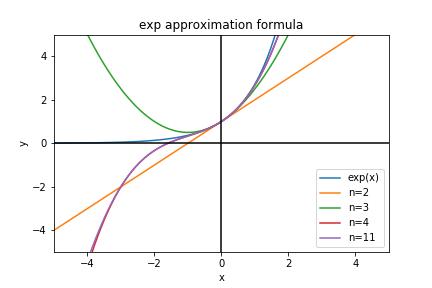
\includegraphics[width=120mm,bb=0 0 432 288]{figures/exp.png}
  \caption{exp関数のマクローリン展開}
\end{figure}
\begin{figure}[H]
\label{im:sine}
  \centering
  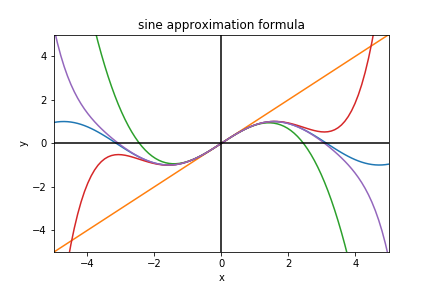
\includegraphics[width=120mm,bb=0 0 432 288]{figures/sine.png}
  \caption{sin関数のマクローリン展開}
\end{figure}

\begin{figure}[H]
\label{im:cosine}
  \centering
  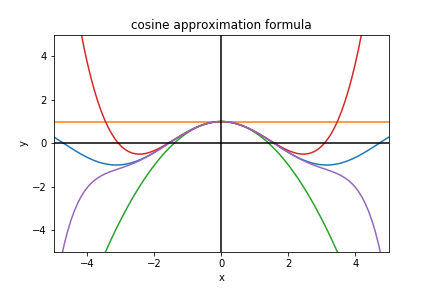
\includegraphics[width=120mm,bb=0 0 432 288]{figures/cosine.png}
  \caption{cos関数のマクローリン展開}
\end{figure}

\begin{eqnarray}
\mathrm{e}^x = \sum_{(k=0)}^\infty \frac{x^k}{x!} = 1 + \frac{x}{1!} + \frac{x^2}{2!} + \frac{x^3}{3!} + ...
\label{eq:sisuu}
\end{eqnarray}

\begin{eqnarray}
\sin x = \sum_{k=0}^{\infty}(-1)^k \frac{x^{2k + 1}}{(2k + 1)!} = \frac{x}{1!} - \frac{x^3}{3!} + \frac{x^5}{5!} - \frac{x^7}{7!} +  ...
\label{eq:sain}
\end{eqnarray}

\begin{eqnarray}
\cos x = \sum_{k=0}^\infty(-1)^k \frac{x^{2k}}{(2k)!} = 1 - \frac{x^2}{2!} + \frac{x^4}{4!} - \frac{x^6}{6!} + ...
\label{eq:cosa}
\end{eqnarray}

賢い人なら気付くかもしれません!!!\\
気付きますよね??\\
気付かないわけがありません.\\
なんとなくですが, 式(\ref{eq:sain})と式(\ref{eq:cosa})を足すと, 式(\ref{eq:sisuu})っぽいですよね!!\\
\\
え?違うじゃんって?\\
うるせえよ, だいたい一緒だろうが.\\
\\
\\
細かいやつは女の子に嫌われるんだぞ!この陰キャが!!\\
\\
陽キャの僕はとりあえず足してみます.
\\
\begin{eqnarray}
\mathrm{e}^x = \sum_{(k=0)}^\infty \frac{x^k}{x!} = 1 + \frac{x}{1!} + \frac{x^2}{2!} + \frac{x^3}{3!} + \frac{x^4}{4!} + ...
\end{eqnarray}
\begin{eqnarray}
\sin x + \cos x = 1 + \frac{x}{1!} - \frac{x^2}{2!} - \frac{x^3}{3!} + \frac{x^4}{4!} + ...
\label{eq:mix}
\end{eqnarray}

うーん, 惜しいですよね. もうちょっと, あとは符号だけ変えちゃえば大丈夫そうなのですが...\\
2項ずつ, 符号があってたりあってなかったりしてますね.\\
\\
これは一寸難しいですね. もし交互に異なるのであれば, 式(\ref{eq:mix})の構成要素のどちらかに -1 をかければ良いのですが, 2項ずつとなるとそうもいきません. かといって両方にマイナスをかけても, 違う形になるし...\\
\\
この段階で, 操作するべきは指数関数と, 三角関数のどちらかという指針がたちます.\\
\\
しかし, そのまま-1をかけても意味がない. そこで式に注目すると, 何乗もしています. なんとか乗した時に符号が変わればいいのですから, ここで虚数単位iの導入に目星をつけます.\\
\\
とりあえず指数の方にやってみましょう.
\begin{eqnarray}
\begin{split}
\mathrm{e}^{ix} \\
& = \sum_{(k=0)}^\infty \frac{ix^k}{x!} = 1 + \frac{ix}{1!} + \frac{i^2x^2}{2!} + \frac{i^3x^3}{3!} + \frac{i^4x^4}{4!} + ...\\
& = 1 + i\frac{x}{1!} - \frac{x^2}{2!} - \frac{ix^3}{3!} + \frac{x^4}{4!} + ...
\label{eq:eix}
\end{split}
\end{eqnarray}
ちょっといい感じですね.\\
次に, 分母が奇数の時にiが残ってしまっているので, 奇数に対応しているsinの方にもiをかけてみましょう!\\
\begin{eqnarray}
i\sin x = \sum_{k=0}^{\infty}(-1)^k \frac{x^{2k + 1}}{(2k + 1)!} = \frac{ix}{1!} - \frac{ix^3}{3!} + \frac{ix^5}{5!} - \frac{ix^7}{7!} +  ...
\end{eqnarray}
問題なさそうですね!改めてcosと足してみます!!\\
\begin{eqnarray}
\cos x + i\sin x = 1 + i\frac{x}{1!} - \frac{x^2}{2!} - \frac{ix^3}{3!} + \frac{x^4}{4!} + ...
\label{eq:cossin}
\end{eqnarray}
式(\ref{eq:eix})と式(\ref{eq:cossin})を見比べると, 見事に一致しています!!!\\
\\
これでオイラーの公式の証明がおわりですね!!\\
\\
オイラーの公式とは, 指数関数と三角関数をマクローリン展開した際にでてきた奴らが似ていたので, 虚数を導入してみたらきれいに等号で結べたねって事です.\\

\subsection{オイラーの公式の有用性}
オイラーの公式とは
\begin{eqnarray}
\mathrm{e}^{i\theta} = \cos \theta + i\sin \theta
\end{eqnarray}
であった.\\
\\
この時, Θにπを代入すると, 更に美しくなります.
\\
\begin{eqnarray}
\mathrm{e}^{i\pi} = -1 + 0\\
\mathrm{e}^{i\pi} + 1 = 0
\end{eqnarray}
実際に計算すれば分かりますね. たしかに成り立ちます. \\
最も基本である数字0と1, そしてネイピア数, 円周率, 虚数...\\
数学において偉大と言われる奴らが一堂に会して, あっさりとまとまっているのです!!!\\
ひええええ...!!!\\
\\
これこそが, オイラーの公式が人類の至宝といわれる所以ですね!\\
\\
\\
さて, オイラーの公式を信号処理の数学にどのように使っていくかというと, ざっくりした流れはこうだ!!!\\
\begin{itemize}
 \item 取得した関数を三角関数の和で表す
 \item 複素平面にもってきて極座標で表す
 \item 極座標を指数関数に変換する
 \item 計算がめっちゃ楽だし, 多次元のデータを取得できる
 \item 色々わかる!!うれしい!!
\end{itemize}
厳密に言うと脳波は定常性をもっていないので三角関数の和で表す事は出来ないんだが, 短時間の窓を設けたりウェーブレットを使う事によってそこは解決できる. \\
とりあえず今は, オイラーの公式を使う事によって脳波を簡単な形で表せる上にいろんな情報を読み取れるようになる!!すごい!!偉大だ!!!\\
\\
だけ分かればいい.\\
次節から実際にフーリエ変換などで使っていくので, オイラーの公式は脳にフィットさせといてください.\\

崇めよ!!!!!\\

\section{フーリエ変換}
さて, いよいよ本節から実際に我々が脳波と戦う際に用いる技の紹介となっていきます. 前章(\ref{basics})が理解できている諸君なら, それほどつまずく事もないはずです. 実際僕は, 前章に値する内容の理解と精査に非常に時間をかけましたが, これ以降はそれほど時間をかけずに理解を進める事が出来ました. 基本を忘れず臨んでください.
\subsection{脳波とは}
そもそも, 解析方法を考える以前に...\\
我々は脳波という似非科学チックな香ばしいものと対峙するわけですが, こいつの特性を知らずに武器や魔法を準備するのは非効率ですね. まずは脳波というものがどういったものなのかを考えてみます. \\
\\
脳波とは, 脳に無数に存在する脳神経細胞が刺激を受け, その総量が閾値を超えた時に発生される電気信号 ... の集合体の事です.\\
\\
領域Aに脳細胞が100万個あったとしましょう. \\
そのうち, 70万個が発火していて, 30万個が沈黙していたとします. 領域A直上にある脳波計の電極は, そこら一帯の電気的活動の総和を観測し, 領域Aで強い活動があったと記すわけです(図\ref{im:topo}).\\
\\
この時の「強い活動」というのは, 電極で計測された電気信号の振幅, 100万の細胞電位の総和の値です. これが大きい程, 強い活動という解釈がされます.\\

\begin{figure}[H]
\label{im:topo}
  \centering
  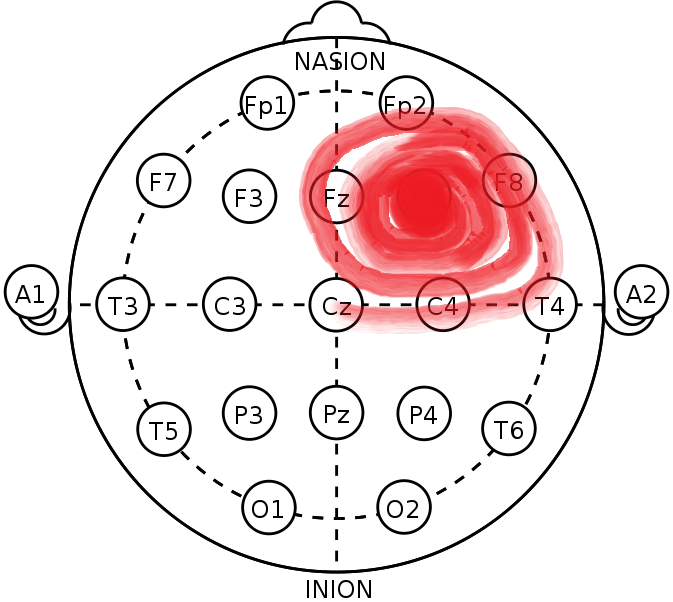
\includegraphics[width=120mm,bb=0 0 673 602]{figures/topomap.png}
  \caption{電極で拾われる脳波のイメージ. 近傍電位の総和}
\end{figure}

しかし, 元来神経細胞の1回の発火は一瞬のものです. 2つの細胞があったとして, それらが数ms間隔で交互に活動しているとしたら, 片方が発火している間にもう片方は負の方向に電位を発しているわけですから, その総和を取ると細胞1個の発火分にも満たない事になります. \\
これは当然, 数百万単位の細胞が集まった時にも同じ事が言えて, 振幅が小さいからといって脳が活動していない ... という訳ではありません. 単に同期的活動を行っているわけではないという事です.\\
\\
本来はパルス波っぽい挙動をする神経信号ですが, それらが無数に存在し, 各々のタイミングで活動をしているため, 脳波計の電極によって計測される信号は連続的で, 非常に複雑な挙動を取る波となります. \\
\\
この波を俗に脳波と言い, 振幅が大きい時には強い活動 (正確には同期した活動) が行われていて, 逆に振幅が小さい時には同期していない, つまり適当な活動を行っているといった解釈がなされたりします. \\
しかしこのままでは, 複雑すぎて人間の目で見たら何がどうなっているのか全く分からず, 麻酔科医やてんかんの診断をする超能力医者のようなスーパーマンでもない限り, 「これは○○の脳波だ!」とか言えません. そこで凡人の我々は, どうにかしてこの複雑怪奇な脳波を解釈し, 脳の活動を解明する必要があるわけです.\\

そこで, 最も基礎となるアプローチが...\\
複雑すぎて分からないなら, 単純な波に分解してあげればいいじゃん??\\ 
というやつです. どんな波も, 直交性をもつ波に分解できるみたいな話題が前章にありましたよね?あれを利用します!!
\\
こうして, 複雑極まりない脳波を, 単純で解釈のしやすい三角関数の足し合わせとして表現しよう!というのがフーリエ変換のモチベーションです.\\

\begin{figure}[H]
\label{im:eeg}
  \centering
  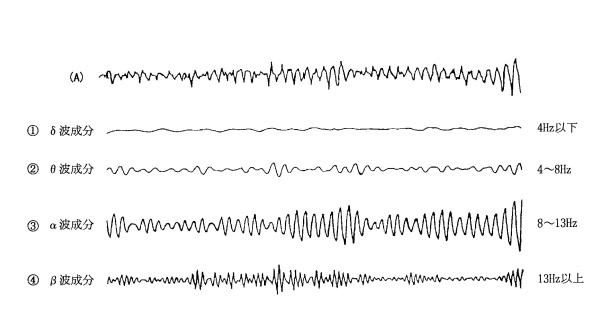
\includegraphics[width=120mm,bb=0 0 600 313]{figures/eeg.jpg}
  \caption{A. 脳波の例 1 ~ 4は周波数帯成分}
\end{figure}

\subsection{フーリエ級数展開}
さて, フーリエ変換をする目的は, 複雑すぎて解釈できない時間関数を単純な関数によって表現する事で表現することでした.\\
\\
複雑な関数でも, 三角関数の足し合わせで表現できるという事は既に確認しましたね. 三角関数の特徴は, その振幅と角周波数が分かれば定義する事ができます. \\
角周波数とは, 1sの間にどれだけの角度波が進むかという指標で, 周波数とかから求める事が出来ます. まあ周波数って考えちゃっても大体おkです. \\
\\
つまりフーリエ変換とは, 元関数を単純な三角関数に分け, それぞれの振幅を角周波数毎に求める事をさします.\\
\\
このうち, 元関数f(t)を単純な三角関数の足し合わせに分解するまでをフーリエ級数展開と言い, 式では以下のようになります. 
\begin{eqnarray}
f(t) = a_0 + \sum_{\omega=1}^\infty {(a_\omega \sin(\omega t) + b_\omega \cos(\omega t))}
\label{eq:fourierkyusu}
\end{eqnarray}
式(\ref{eq:fourierkyusu})の意味はこうです. 「元関数f(t)を, 1から無限の角周波数のsin, cos波の足し合わせとして表現する」 そのまんまですね!\\
\\
ここでのaやbは変数で, 実際にはそれぞれの項毎に異なる値を取ります. 要は振幅の事ですね.\\
\subsection{複素フーリエ級数}
しかし, 式(\ref{eq:fourierkyusu})は面倒ですね. なんていったってsinとcosを分けて計算するのがだるすぎます. どうにか綺麗にできないものか...\\
\\
え?オイラーの公式を使えばいいって? ...天才かよ!!
\\
早速オイラーの公式を使って簡単にしてみましょう. 
\begin{eqnarray}
\mathrm{e}^{i\omega t} = \cos\omega t + i\sin\omega t
\label{eq:normaleuler}
\end{eqnarray}
いつもは$\pi$のところですが, 今回は空気を読んで角周波数$\omega t$に変形しています. しかし問題はあれです. オイラーの公式には愛がありますが, フーリエ級数展開の方には愛がありません. どうしたことか.\\
\\
オイラーの公式の裏を使います.
\begin{eqnarray}
\mathrm{e}^{-i\omega t} = \cos\omega t - i\sin\omega t
\label{eq:eulerminus}
\end{eqnarray}
式(\ref{eq:eulerminus})が成り立つのは大丈夫ですね?角度が実軸対称に飛んだら, cos成分は変わりませんがsin成分は符号が反転します. うちの猫でも知ってる事です.\\
\\
さて, 次に式(\ref{eq:normaleuler})と式(\ref{eq:eulerminus})を連立して解く事で式(\ref{eq:fourierkyusu})のcosとsinを置き換えます. \\
\begin{eqnarray}
f(t) = a_0 + \sum_{\omega=1}^\infty {(a_\omega \frac{\mathrm{e}^{i\omega t}+\mathrm{e}^{-i\omega t}}{2} + b_\omega \frac{\mathrm{e}^{i\omega t} - \mathrm{e}^{-i\omega t}}{2i})}
\label{eq:complexfourier}
\end{eqnarray}
この式を同類項を抜き出して整理すると
\begin{eqnarray}
f(t) = a_0 + \sum_{\omega=1}^\infty {(\frac{a_\omega - ib_\omega}{2}\mathrm{e}^{i\omega t})} + \sum_{\omega=1}^\infty {(\frac{a_\omega + ib\omega}{2}\mathrm{e}^{i\omega t})}
\label{eq:complexfourierkai}
\end{eqnarray}
となり, 更に$\mathrm{e}^{-i\omega t}$において$\omega$を1から$\infty$まで足すのと, $\mathrm{e}^{i\omega t}$において$-\infty$から-1まで足すのは同義なため(図を書けばわかる), この3項をうまくくっつける事で
\begin{eqnarray}
f(t) = \sum_{\omega = -\infty}^\infty F_\omega \mathrm{e}^{i\omega t}
\end{eqnarray}
とおけますね!いい感じにまとまりました!!!\\
あ, 定数部分は面倒なので$F_\omega$とおいてます. \\
\\
フーリエ変換では, この係数たちを求めます. 
\subsection{フーリエ変換} 
実際に式を見てみましょう.\\
\begin{eqnarray}
F(\omega) = \int_{-\infty}^{\infty} f(t)\mathrm{e}^{-i\omega t}
\label{eq:furier}
\end{eqnarray}

です. さっそく式(\ref{eq:furier})を解読してみましょう. 大丈夫. 基礎がしっかりできている人なら自ずと理解できるはずです.\\
\\
まず, eの肩に $ -i\omega t $ が載っていますね. この形はどこかで見た事があります. そう, オイラーの公式ですね!!\\
オイラーの公式にマイナスをかけたやつです. つまり $ \cos\omega t  - i\sin\omega t $ ですね. \\
式(\ref{eq:furier})は以下の式に変形できそうです.\\
\begin{eqnarray}
F(\omega) = \int_{-\infty}^{\infty} f(t)(\cos\omega t - i\sin\omega t)
\label{eq:furierkai}
\end{eqnarray}
おお、結構読めてきたんじゃないですかね.\\
分配法則が分からない輩のために, 更に式(\ref{eq:furierkai})を変形します.\\
\begin{eqnarray}
F(\omega) = \int_{-\infty}^{\infty} (f(t)\cos\omega t - f(t)i\sin\omega t)
\label{eq:furierkaikai}
\end{eqnarray}
もう完璧ですね. ここまで解してあげれば赤ちゃんでも噛み砕けそうです!!噛み砕けない人は乳歯が生えていないのでしょう. かわいそうに...\\
\\
さて, 式(\ref{eq:furierkaikai})を日本語にしてみましょうか.\\
まず, 時間(t)における元関数(ここでは, ある電極で取れた脳波ですね)と, 角周波数($\omega$)のcos, sin成分それぞれとの内積を取っています. 
\\
フーリエ変換において求めたい係数とは, 「元関数がその角周波数($\omega$)の三角関数に如何に似てるか」の指標です. そして関数の類似度の指標は内積で表せるんでしたね!!\\
\\
次に, sin成分が負($\mathrm{e}^{-i\omega t}$)になっている理由です. 内積とは「似ている度」の指標ですね. 普通の数字やベクトルでしたら正の値になりますが, 今回のように虚数や複素数の場合は内積の結果が複素数の形をとってしまう事になります.\\
それだと解釈に困りますね?どうにかして虚数成分は消えた感じの結果が欲しいわけです. 虚数成分を消す...共役複素数を使えばいいですね!!!\\
\\
これにより, ある角周波数成分 $\mathrm{e}^{i\omega t}$と元関数f(t)の内積を求める際に$\mathrm{e}^{-i\omega t}$を用いるわけです. まあ, やってるのは普通に内積です.\\
\\
\\
内積とは, 「どれだけ似ているか」の指標でしたね. つまりここで, 元関数は角周波数($\omega$)の三角関数とどれだけ似ているかを見ているわけです!!\\
そしてその結果を $-\infty$ から$\infty$ までの範囲で積分 ... 足し算しています.\\
この値がF($\omega$)らしいですね. さて, こいつはどういった条件でどういった値を取るかというと, 元関数の中に角周波数($\omega$)の成分が多ければ多い程, 内積の値は1に近くなります. という事はその総和も大きくなります. 逆に値が小さいという事は内積の値も小さい ... つまり元関数の中に角周波数($\omega$)の成分は少ないという事になりますね!!\\
\\
こうして, 複雑怪奇な時間関数を周波数関数に変換(というか見方を変える)事によって, より解釈のしやすい形に変換するのがフーリエ変換の強みです.\\
\\
\subsection{フーリエ変換の実用}
実際には, 式(\ref{eq:furier})によって無限の周波数成分を抜き出し, それぞれの振幅を求める事で, 元関数(t)はそれぞれの周波数をそれぞれの振幅倍したsin波の足し合わせで出来てるね!と解釈します.\\
例えば, 「タスク1をやらせた時の被験者君は5 -- 7Hzくらいの脳波がよくでているね!」「タスク2の時には大して強くないね。てことはタスク1と5 --7Hzの脳波には何か関係がありそうだね!!」といった具合です. 論文にもそのまんま書かれています.
\\
人はこれを周波数分解といい, これを使った解析が周波数解析だとかスペクトル解析と呼ばれる種々の解析になります!!(上の「」に入ってるのも周波数解析による解釈)
\section{wavelet 変換}
\subsection{フーリエ変換の弱点}
万能に思えるフーリエ変換ですが, 実は弱点があります.
\subsection{morlet wavelet}
\end{document}